\documentclass{article}


%pacchetti extra da scaricare dblfloatfix, fancyhdr
\usepackage{fancyhdr}%creazione header-footer
\usepackage{graphicx} %serve per inserire immagini
%\usepackage{dblfloatfix} %serve per posizionare gli elementi dove si vuole
\usepackage[hidelinks]{hyperref} %serve per i link
\usepackage{tikz}
% \usepackage{tgadventor} % font
\usepackage[useregional=numeric,showseconds=true,showzone=false]{datetime2}
\usepackage{caption}
\usepackage{geometry}
\usepackage{setspace}
\usepackage{eurosym}
\usepackage[italian]{babel}
\usepackage[hidelinks]{hyperref}
\usepackage{tabularx}
\usepackage{longtable}
\usepackage{float}

\usepackage{graphicx}
% Margini della pagina
\geometry{a4paper, margin=1in}

% Intestazione personalizzata
\pagestyle{fancy}
\fancyhf{}
\fancyhead[L]{Code7Crusaders - Software Development Team}
\fancyhead[R]{\thepage}

% Spaziatura delle righe
\setstretch{1.2}

\begin{document}

\begin{titlepage} 

    \AddToHookNext{shipout/background}{
    \begin{tikzpicture}[remember picture,overlay]
    \node at (current page.center) {
    
\includegraphics{../../../img/background.png}
    };
    \end{tikzpicture}
    }

    \centering
    \vspace*{2cm}
    
    
\includegraphics[width=0.3\textwidth]{../../../img/logo/7Crusaders_logo.png} % Aggiungi il logo qui
    \vspace{1cm}
    
    {\Huge \textbf{Code7Crusaders}}\\
    \vspace{0.5cm}
    {\Large Software Development Team}\\
    \vspace{2cm}
    
    \large \textbf{Analisi Dei Requisiti}
    \vspace{3.9cm}

    \textbf{Membri del Team:}\\
    Enrico Cotti Cottini, Gabriele Di Pietro, Tommaso Diviesti \\
    Francesco Lapenna, Matthew Pan, Eddy Pinarello, Filippo Rizzolo \\
    \vspace{0.5cm}
    
    \vspace{1cm}
\end{titlepage}



\newpage
%------------------------Versioni
\begin{table}[h]
    \centering
    \renewcommand{\arraystretch}{1.2}
    \setlength{\tabcolsep}{5pt}
    \begin{tabular}{|c|c|c|c|m{0.35\textwidth}|}
        \hline
        \textbf{Ver} & \textbf{Data} & \textbf{Redattore} & \textbf{Verificatore} & \textbf{Descrizione} \\
        \hline
        2.3 & 6/03/2025 & Gabriele Di Pietro & Tommaso Diviesti & Rimosso U.C.6.5, aggiunta sezione 4.9, aggiornati Requisiti secondo il verbale esterno 4/03/25 \\
        \hline
        2.2 & 5/03/2025 & Eddy Pinarello & Tommaso Diviesti & Aggiornamento dei requisiti funzionali dopo negoziazione con l'azienda \\
        \hline
        2.1 & 28/02/2025 & Enrico Cotti Cottini & Gabriele Di Pietro &  Aggiornamento requisiti funzionali e tracciamenti relativi, definito U.C.23, correzione stesura U.C.2.1 \\
        \hline
        2.0 & 19/02/2025 & Enrico Cotti Cottini & Gabriele Di Pietro & Approvazione documento  \\
        \hline
        1.7 & 18/02/2025 & Enrico Cotti Cottini & Eddy Pinarello & Aggiunti requisiti qualitativi e di vincolo per il Piano di Qualifica \\
        \hline
        1.6 & 18/02/2025 & Enrico Cotti Cottini & Eddy Pinarello & Aggiunti nuovi requisiti funzionali e di vincolo per la gestione del chatbot e delle metriche. Integrazione con modelli di embedding e LangChain. Aggiunti requisiti RFO43, RFD44, RFD45, RFO46, RVO18, RVD19, RVO20 nel tracciamento \\
        \hline
        1.5 & 17/02/2025 & Eddy Pinarello & Enrico Cotti Cottini & Rivisti requisiti di vincolo, corretti requisiti errati, implementati requisiti sulle tecnologie, tracciati nuovi casi d'uso \\
        \hline
        1.4 & 15/02/2025 & Gabriele Di Pietro & Enrico Cotti Cottini & Aggiunto tracciamento Caso d'uso - Requisito \\
        \hline
        1.3 & 14/02/2025 & Filippo Rizzolo & Enrico Cotti Cottini & Correzione del caso d'uso U.C.20 \\
        \hline
        1.2 & 11/02/2025 & Filippo Rizzolo & Enrico Cotti Cottini & Correzione dei casi d'uso U.C.14, U.C.15 e U.C.17 \\
        \hline
        1.1 & 10/02/2025 & Gabriele Di Pietro & Filippo Rizzolo & Prima stesura del documento dopo correzioni Colloquio RTB \\
        \hline
        1.0 & 04/02/2025 & Gabriele Di Pietro & Tommaso Divesti & Correzione imprecisioni e approvazione documento \\
        \hline
        0.8 & 27/01/2025 & Gabriele Di Pietro & Eddy Pinarello & Correzioni casi d'uso e aggiunti nuovi requisiti \\
        \hline
        0.7 & 14/01/2025 & Gabriele Di Pietro & Enrico Cotti Cottini & Aggiunte tabelle requisiti \\
        \hline
        0.6 & 17/12/2024 & Enrico Cotti Cottini & Eddy Pinarello & Ridefinizione dell'architettura dopo un'analisi approfondita dei mezzi \\
        \hline
        0.5 & 16/12/2024 & Gabriele Di Pietro & Enrico Cotti Cottini & Inizio stesura requisiti \\
        \hline
        0.3 & 06/12/2024 & Gabriele Di Pietro & Enrico Cotti Cottini & Aggiunti casi d'uso \\
        \hline
        0.2 & 20/11/2024 & Enrico Cotti Cottini & Gabriele Di Pietro & Prima stesura del documento \\
        \hline
    \end{tabular}
\end{table}

%----------------

\newpage
\tableofcontents
\listoftables
\listoffigures

\newpage

\section{Introduzione}

\subsection{Scopo del documento}
Questo documento ha lo scopo di definire le regole e le procedure che ogni membro del team deve seguire durante 
lo sviluppo del progetto. In particolare, mira a stabilire il \textit{Way of Working} del gruppo. 

La sua redazione inizia nelle prime fasi del progetto e continua anche durante le fasi successive, 
per essere costantemente aggiornato e adattato alle esigenze del team. 

Il processo seguirà le linee guida dello standard ISO/IEC 12207:1995, suddivise in:
\begin{itemize}
    \item Processi primari
    \item Processi di supporto
    \item Processi organizzativi
\end{itemize}


\subsection{Scopo del progetto}
Il progetto si propone di sviluppare un Assistente Virtuale intelligente per aziende che operano nel 
settore della vendita multiprodotto. Questo assistente avrà il compito di semplificare l'accesso alle 
informazioni sui prodotti disponibili, rispondendo alle domande più frequenti poste dai clienti in modo rapido ed efficace.

Grazie all'uso di tecnologie avanzate come il \href{https://code7crusaders.github.io/docs/RTB/documentazione_interna/glossario.html#machine-learning}{Machine Learning\textsuperscript{G}} e il \href{https://code7crusaders.github.io/docs/RTB/documentazione_interna/glossario.html#natural-language-processing-nlp}{Natural Language Processing\textsuperscript{G}}, 
il sistema sarà in grado di analizzare i dati contenuti nei cataloghi aziendali e negli archivi digitali, 
fornendo risposte precise e personalizzate.

L’obiettivo principale è ridurre la dipendenza dagli specialisti aziendali, che attualmente rappresentano 
l’unico canale di accesso per ottenere dettagli approfonditi sui prodotti. Questo migliorerà l’efficienza 
operativa, ottimizzerà le risorse e offrirà una migliore esperienza ai clienti, che potranno interagire con 
il sistema in modo intuitivo e diretto attraverso piattaforme digitali come siti web o chatbot.

In sintesi, il progetto intende rendere l'accesso alle informazioni aziendali più semplice, veloce e scalabile, 
migliorando al contempo la qualità del servizio offerto ai clienti.


\subsection{Glossario}
Per evitare ambiguità e facilitare la comprensione del documento, si farà uso di un glossario, 
contenente la definizione dei termini tecnici e degli acronimi utilizzati, 
che sarà incluso all'interno del file \textit{glossario}.


\subsection{Riferimenti}
\subsubsection{Normativi}
\begin{itemize}
	\item \textbf{Capitolato C7:} \\ \url{https://www.math.unipd.it/~tullio/IS-1/2024/Progetto/C7.pdf}
	\item \textbf{ISO/IEC 12207:1995} \\ \url{https://www.math.unipd.it/~tullio/IS-1/2009/Approfondimenti/ISO_12207-1995.pdf}
\end{itemize}

\subsubsection{Informativi}
\begin{itemize}
    \item\textbf{Glossario RTB}\\ \url{https://code7crusaders.github.io/docs/RTB/documentazione_interna/glossario.html}
    \item\textbf{Documentazione Git}\\ \url{https://git-scm.com/docs}
    \item\textbf{Documentazione Latex}\\ \url{https://www.latex-project.org/help/documentation/}

\end{itemize}


\newpage

\section{Descrizione del prodotto}

\subsection{Obiettivi del prodotto}
Il progetto ha come obiettivo la realizzazione di una piattaforma che consenta di 
gestire un assistente virtuale per la conoscenza e la descrizione di bevande, 
sfruttando un’infrastruttura basata su modelli linguistici di grandi dimensioni. 
La piattaforma dovrà supportare le richieste degli utenti in modo rapido, 
preciso e sempre disponibile, eliminando la necessità di uno specialista fisico. 
Essa permetterà la consultazione di informazioni dettagliate su prodotti come caratteristiche, 
formati disponibili e suggerimenti d’uso, adattandosi alle esigenze specifiche 
dei clienti e garantendo un’interazione fluida in linguaggio naturale. 
L’assistente virtuale sarà progettato per integrarsi con database aziendali, 
sfruttando le informazioni esistenti per rispondere alle domande in modo 
contestualizzato e accurato.

\subsection{Architettura del prodotto}
I componenti del prodotto sono:
\begin{itemize}
    \item \href{https://code7crusaders.github.io/docs/RTB/documentazione_interna/glossario.html#database-relazionale}{\textbf{Database Relazionale}\textsuperscript{G}}:  
    Questo componente memorizza i dati strutturati dell’azienda, come descrizioni di prodotti, ingredienti, specifiche tecniche e altro. È il punto di partenza per acquisire informazioni utili che saranno processate e utilizzate dal sistema. Supporta query SQL per consentire l'accesso rapido e organizzato ai dati.
    
    \item \href{https://code7crusaders.github.io/docs/RTB/documentazione_interna/glossario.html#embedding}{\textbf{Embedding\textsuperscript{G}} } \textbf{Model}:  
    L’Embedding Model è un modello pre-addestrato in grado di trasformare il testo in rappresentazioni numeriche preservando il significato semantico. Viene utilizzato sia per i dati aziendali durante l’addestramento che per le domande poste dagli utenti. Gli embedding risultanti permettono confronti efficienti nel \href{https://code7crusaders.github.io/docs/RTB/documentazione_interna/glossario.html#database-vettoriale}{database vettoriale\textsuperscript{G}}.
    
    \item \href{https://code7crusaders.github.io/docs/RTB/documentazione_interna/glossario.html#database-vettoriale}{\textbf{Database Vettoriale}\textsuperscript{G}}:  
    Questo componente archivia i vettori generati dall’\href{https://code7crusaders.github.io/docs/RTB/documentazione_interna/glossario.html#embedding}{Embedding\textsuperscript{G}} Model. Utilizza indicizzazione ottimizzata per operazioni di \href{https://code7crusaders.github.io/docs/RTB/documentazione_interna/glossario.html#nearest-neighbor-search-nns}{\textit{nearest neighbor search}\textsuperscript{G}}, permettendo di trovare rapidamente i vettori più simili a una query. È il cuore della fase di recupero delle informazioni nel sistema.
    
    \item \href{https://code7crusaders.github.io/docs/RTB/documentazione_interna/glossario.html#llm-large-language-model}{\textbf{LLM}\textsuperscript{G}}:  
    Il Large Language Model riceve in input il contesto fornito dal \href{https://code7crusaders.github.io/docs/RTB/documentazione_interna/glossario.html#database-vettoriale}{database vettoriale\textsuperscript{G}} e la domanda dell’utente. Grazie alla sua capacità generativa, l'\href{https://code7crusaders.github.io/docs/RTB/documentazione_interna/glossario.html#llm-large-language-model}{LLM\textsuperscript{G}} riceve in input il contesto fornito dal database vettoriale e la domanda dell’utente. Grazie alla sua capacità generativa, il LLM elabora risposte dettagliate e accurate, combinando i dati presenti con la comprensione del linguaggio naturale.
    
    \item \textbf{Web App}:  
    La Web App è l’interfaccia attraverso la quale gli utenti interagiscono con il sistema. Fornisce un’esperienza semplice e intuitiva per inserire domande e visualizzare risposte. Comunica con il backend tramite \href{https://code7crusaders.github.io/docs/RTB/documentazione_interna/glossario.html#api-rest-representational-state-transfer}{API REST\textsuperscript{G}} per garantire un'interazione rapida e scalabile.
\end{itemize}

\subsection{Implementazione scelta: LLM e strumenti}
\subsubsection{Scelta dell'LLM}
Dopo un'attenta analisi comparativa tra i modelli di Huggingface (BLOOM e varianti) e OpenAI (GPT-4o e GPT-4omini) nel file di \textbf{analisi modelli.pdf}, si è optato per l'utilizzo di GPT-4omini di OpenAI. La scelta è motivata dai seguenti fattori:
\begin{itemize}
    \item \textbf{Prestazioni}: GPT-4omini offre risultati superiori rispetto ai modelli open-source in termini di accuratezza e capacità di generazione del linguaggio, come evidenziato dai \href{https://code7crusaders.github.io/docs/RTB/documentazione_interna/glossario.html#benchmark}{benchmark\textsuperscript{G}} \textbf{analisi modelli}.
    \item \href{https://code7crusaders.github.io/docs/RTB/documentazione_interna/glossario.html#scalabilità}{\textbf{Scalabilità}\textsuperscript{G}}: Le API di OpenAI garantiscono un'infrastruttura cloud scalabile, eliminando i costi e la complessità legati alla gestione locale di modelli di grandi dimensioni.
    \item \textbf{Costi ottimizzati}: Il costo basato sui \href{https://code7crusaders.github.io/docs/RTB/documentazione_interna/glossario.html#token}{token\textsuperscript{G}} elaborati permette un utilizzo flessibile e sostenibile, adattandosi alle esigenze di carico variabile del sistema.
    \end{itemize}
    Per ulteriori informazioni di confronto tra i vari Modelli visitare il seguente link:
    \href{https://code7crusaders.github.io/docs/altri_documenti/analisi_modelli_firmato.html}{\textit{\underline{Analisi Modelli LLM}}}


\subsubsection{Pipeline di Implementazione}
L'implementazione sfrutta un'architettura RAG (Retrieval-Augmented Generation), integrando i seguenti componenti:
\begin{enumerate}
    \item Generazione degli Embedding: Le informazioni aziendali (es. cataloghi di prodotti) vengono preprocessate e trasformate in vettori numerici tramite \href{https://code7crusaders.github.io/docs/RTB/documentazione_interna/glossario.html#bert-bidirectional-encoder-representations-from-transformers}{BERT\textsuperscript{G}} \href{https://code7crusaders.github.io/docs/RTB/documentazione_interna/glossario.html#embedding}{Embedding\textsuperscript{G}}: Le informazioni aziendali (es. cataloghi di prodotti) vengono preprocessate e trasformate in vettori numerici tramite BERT di Huggingface.
    \item Archiviazione degli \href{https://code7crusaders.github.io/docs/RTB/documentazione_interna/glossario.html#embedding}{Embedding\textsuperscript{G}}: I vettori generati vengono memorizzati e indicizzati utilizzando \href{https://code7crusaders.github.io/docs/RTB/documentazione_interna/glossario.html#faiss}{FAISS\textsuperscript{G}}, che consente un recupero efficiente dei dati rilevanti.
    \item Integrazione con LLM: Le domande degli utenti, trasformate in embedding, vengono confrontate con il \href{https://code7crusaders.github.io/docs/RTB/documentazione_interna/glossario.html#database-vettoriale}{database vettoriale\textsuperscript{G}}. Il contesto recuperato viene passato a GPT-4omini per generare risposte accurate e personalizzate.
    \item Web App e \href{https://code7crusaders.github.io/docs/RTB/documentazione_interna/glossario.html#api-rest-representational-state-transfer}{API REST\textsuperscript{G}}: La comunicazione tra frontend (React) e backend avviene tramite \href{https://code7crusaders.github.io/docs/RTB/documentazione_interna/glossario.html#api-rest-representational-state-transfer}{API REST\textsuperscript{G}}, garantendo tempi di risposta rapidi.
\end{enumerate}

\subsubsection{Motivazione degli Strumenti Scelti}
\begin{itemize}
    \item \textbf{BERT + FAISS}: Permette di ottimizzare la fase di retrieval, migliorando l’efficienza della ricerca semantica.
    \item \textbf{GPT-4omini}: Offre risposte di alta qualità con costi prevedibili, bilanciando prestazioni e budget di progetto.
    \item \href{https://code7crusaders.github.io/docs/RTB/documentazione_interna/glossario.html#langchain}{\textbf{LangChain}\textsuperscript{G}}: Facilita l’orchestrazione dell'intera pipeline RAG, riducendo i tempi di sviluppo e semplificando l’integrazione dei componenti.
\end{itemize}

Questa architettura garantisce un sistema performante, flessibile e scalabile, in grado di soddisfare le esigenze degli utenti finali e delle aziende committenti.

\begin{enumerate}
    \item Il sistema riceve in ingresso i dati aziendali strutturati (es. descrizioni, ingredienti).
    \item I documenti vengono pre-processati e suddivisi in blocchi di dati.
    \item I blocchi di testo sono trasformati in vettori numerici tramite l'\href{https://code7crusaders.github.io/docs/RTB/documentazione_interna/glossario.html#embedding}{Embedding\textsuperscript{G}} Model.
    \item I vettori generati sono memorizzati nel \href{https://code7crusaders.github.io/docs/RTB/documentazione_interna/glossario.html#database-vettoriale}{Database Vettoriale\textsuperscript{G}} e indicizzati.
\end{enumerate}
\newpage
\section*{Flusso di Interazione con l'Utente}

\begin{enumerate}
    \item L'utente invia una domanda tramite la Web App.
    \item La domanda viene inoltrata al Web Server tramite \href{https://code7crusaders.github.io/docs/RTB/documentazione_interna/glossario.html#api-rest-representational-state-transfer}{API REST\textsuperscript{G}}.
    \item L'\href{https://code7crusaders.github.io/docs/RTB/documentazione_interna/glossario.html#embedding}{Embedding\textsuperscript{G}} Model trasforma la domanda in un vettore numerico.
    \item Il vettore della domanda viene confrontato con i vettori nel \href{https://code7crusaders.github.io/docs/RTB/documentazione_interna/glossario.html#database-vettoriale}{Database Vettoriale\textsuperscript{G}}.
    \item Viene restituito il contesto più rilevante, insieme alla domanda, all'\href{https://code7crusaders.github.io/docs/RTB/documentazione_interna/glossario.html#llm-large-language-model}{LLM\textsuperscript{G}}.
    \item L'\href{https://code7crusaders.github.io/docs/RTB/documentazione_interna/glossario.html#llm-large-language-model}{LLM\textsuperscript{G}} elabora la risposta utilizzando il contesto fornito.
    \item La risposta viene inoltrata al dispositivo dell'utente tramite \href{https://code7crusaders.github.io/docs/RTB/documentazione_interna/glossario.html#api-rest-representational-state-transfer}{API REST\textsuperscript{G}}.
\end{enumerate}

\begin{figure}[h]
    \centering
    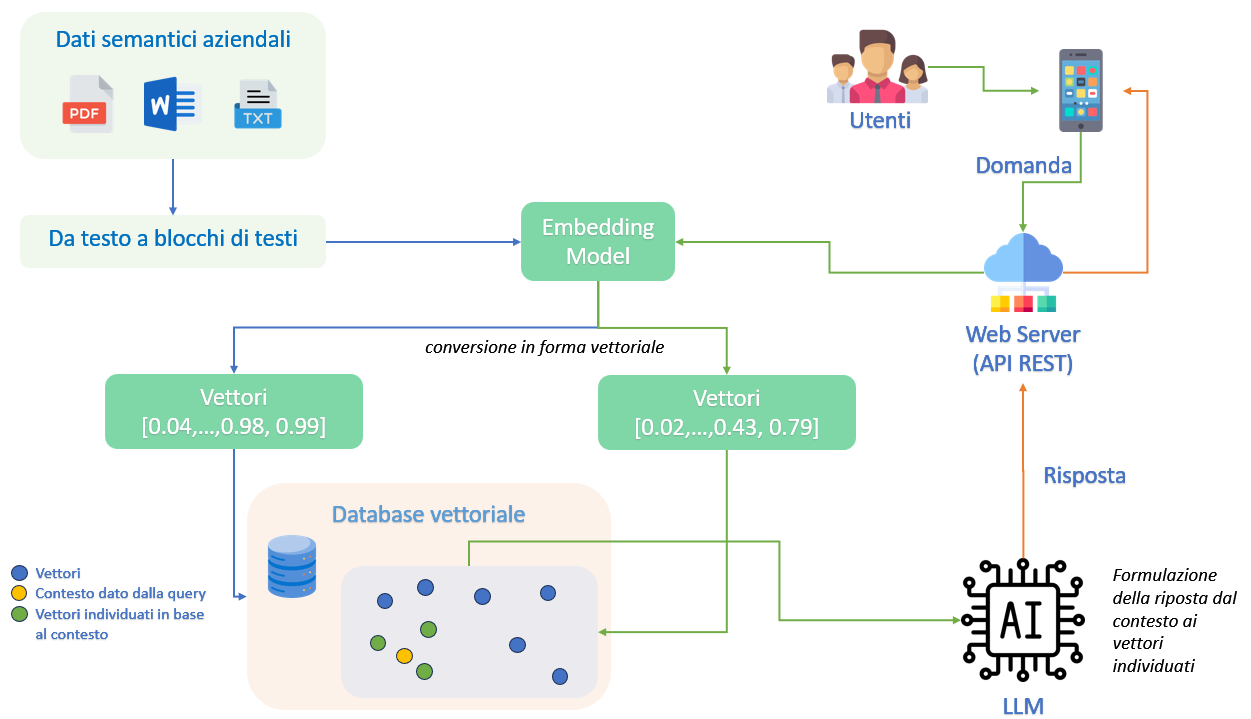
\includegraphics[width=0.8\textwidth]{img/architettura.png}
    \caption{Architettura del prodotto}
    \label{fig:architettura}
\end{figure}

\subsection{Funzionalità del prodotto}
Il prodotto avrà il compito di interagire con i propri utenti attraverso una webapp, rispondendo a domande su cataloghi di bevande. Ogni risposta sarà generata in linguaggio naturale, elaborando i dati tramite \href{https://code7crusaders.github.io/docs/RTB/documentazione_interna/glossario.html#llm-large-language-model}{\textbf{LLM}\textsuperscript{G}}. Le funzionalità principali includono:
\begin{itemize}
    \item \textbf{Interfaccia utente interattiva}: consente agli utenti di porre domande sul catalogo (\textit{es. descrizione di un prodotto o disponibilità in magazzino}) e di ricevere risposte immediate.
    \item \textbf{Motore di ricerca intelligente}: utilizza un sistema di \href{https://code7crusaders.github.io/docs/RTB/documentazione_interna/glossario.html#embedding}{embedding\textsuperscript{G}} per trovare corrispondenze semantiche tra le domande degli utenti e i dati aziendali, estrae il contesto dai dati aziendali per fornire all'\href{https://code7crusaders.github.io/docs/RTB/documentazione_interna/glossario.html#llm-large-language-model}{LLM\textsuperscript{G}} dati accurati da elaborare.
    \item \textbf{Gestione dei dati}: accesso ai dettagli dei prodotti memorizzati in database relazionali, garantendo aggiornamenti in tempo reale. Costruzione di un \href{https://code7crusaders.github.io/docs/RTB/documentazione_interna/glossario.html#database-vettoriale}{database vettoriale\textsuperscript{G}} per l'\href{https://code7crusaders.github.io/docs/RTB/documentazione_interna/glossario.html#embedding}{embedding\textsuperscript{G}} delle parole.
    \item \textbf{Personalizzazione tramite backend}: gli amministratori possono configurare risposte predefinite(\href{https://code7crusaders.github.io/docs/RTB/documentazione_interna/glossario.html#template}{template\textsuperscript{G}} di domanda e risposta), monitorare l’utilizzo e migliorare il sistema tramite feedback utente.
    \item \textbf{Apprendimento continuo}: il sistema evolve grazie ai feedback raccolti dagli utenti, migliorando la qualità delle risposte.
    \item \textbf{Compatibilità multi-dispositivo}: la piattaforma è progettata per essere accessibile 24/7 da mobile e desktop.
\end{itemize}

Il prodotto garantirà inoltre \href{https://code7crusaders.github.io/docs/RTB/documentazione_interna/glossario.html#scalabilità}{scalabilità\textsuperscript{G}} e flessibilità, adattandosi a un’ampia gamma di aziende che desiderano offrire ai propri clienti un’esperienza di interazione avanzata e intuitiva.


\subsection{Tecnologie utilizzate}
Le tecnologie selezionate per la realizzazione del prodotto software sono le seguenti:

\begin{itemize}

    \item \textbf{Embedding Model}: \href{https://code7crusaders.github.io/docs/RTB/documentazione_interna/glossario.html#bert-bidirectional-encoder-representations-from-transformers}{BERT\textsuperscript{G}}\href{https://code7crusaders.github.io/docs/RTB/documentazione_interna/glossario.html#embedding}{\textbf{Embedding\textsuperscript{G}} Model}: BERT (Huggingface) oppure modelli di embedding di Openai (es. Embedding-large) per la trasformazione del testo in vettori semantici. Questo modello viene utilizzato per generare \href{https://code7crusaders.github.io/docs/RTB/documentazione_interna/glossario.html#embedding}{embedding\textsuperscript{G}} efficaci nella fase RAG (Retrieval-Augmented Generation).
    \item \href{https://code7crusaders.github.io/docs/RTB/documentazione_interna/glossario.html#database-relazionale}{\textbf{Database Relazionale}\textsuperscript{G}}: \href{https://code7crusaders.github.io/docs/RTB/documentazione_interna/glossario.html#postgresql}{\textit{PostgreSQL}\textsuperscript{G}} per memorizzare i dati strutturati come cataloghi di prodotti, descrizioni e metadati.
    \item \href{https://code7crusaders.github.io/docs/RTB/documentazione_interna/glossario.html#database-vettoriale}{\textbf{Database Vettoriale}\textsuperscript{G}}: \href{https://code7crusaders.github.io/docs/RTB/documentazione_interna/glossario.html#faiss}{\textit{FAISS}\textsuperscript{G}} per l'archiviazione e il recupero veloce degli embedding e permette un'indicizzazione ottimizzata per la \href{https://code7crusaders.github.io/docs/RTB/documentazione_interna/glossario.html#nearest-neighbor-search-nns}{\textit{nearest neighbor search}\textsuperscript{G}}.
    \item \href{https://code7crusaders.github.io/docs/RTB/documentazione_interna/glossario.html#llm-large-language-model}{\textbf{LLM}\textsuperscript{G}}: OpenAI GPT-4, integrato tramite API OpenAI, per garantire prestazioni elevate e costi scalabili.

\end{itemize}
\begin{figure}[H]

    \centering
    
\includegraphics[width=0.2\textwidth]{img/openai-lockup.png}
    \caption{Logo di OpenAI}
    \label{fig:openai_logo}

\end{figure}

\begin{itemize}
    \item \textbf{Web App}: \textit{React} per lo sviluppo dell’interfaccia utente, combinata con \href{https://code7crusaders.github.io/docs/RTB/documentazione_interna/glossario.html#api-rest-representational-state-transfer}{API REST\textsuperscript{G}} per una comunicazione efficiente con il \href{https://code7crusaders.github.io/docs/RTB/documentazione_interna/glossario.html#backend}{backend\textsuperscript{G}}.
    \item \href{https://code7crusaders.github.io/docs/RTB/documentazione_interna/glossario.html#langchain}{\textbf{LangChain}\textsuperscript{G}}: Libreria di orchestrazione utilizzata per integrare \href{https://code7crusaders.github.io/docs/RTB/documentazione_interna/glossario.html#llm-large-language-model}{LLM\textsuperscript{G}}, database vettoriali e pipeline di retrieval.
\end{itemize}

\begin{figure}[H]
    \centering
    
\includegraphics[width=0.2\textwidth]{img/lang-chain.png}
    \caption{Logo di LangChain}
    \label{fig:langchain_logo}
\end{figure}


\subsection{Utenti finali}
Il prodotto è rivolto a aziende che desiderano offrire un servizio di assistenza 
clienti automatizzato e personalizzato. Gli utenti finali sono quindi i clienti 
delle aziende che interagiranno con l’assistente virtuale per ottenere 
informazioni sui prodotti e ricevere supporto.

\newpage

\section{Casi d'uso}
\subsection{Introduzione}
In questa sezione vengono presentati i casi d'uso individuati durante l'attività di analisi, 
condotta a partire dal capitolato d'appalto e dagli incontri con il proponente. 
Gli attori vengono identificati in base alla gerarchia trovata e 
alle funzionalità potenziali rilevate.

\subsubsection{Codifica dei casi d'uso}
I casi d'uso sono codificati utilizzando la seguente notazione:

\begin{itemize}
    \item \textbf{UC[ID-Principale][ID-Sottocaso]}: Identificativo univoco del caso d'uso, composto da un ID principale che identifica il caso principale e, se necessario, da un ID del sottocaso.
    \item \textbf{Titolo}: Breve descrizione del caso d'uso.
    \item \textbf{Attori}: Elenco degli attori coinvolti nel caso d'uso.
    \item \textbf{Precondizioni}: Condizioni che devono essere vere prima che il caso d'uso possa iniziare.
    \item \textbf{Postcondizioni}: Condizioni che devono essere vere dopo che il caso d'uso è stato completato con successo.
    \item \textbf{Scenario principale}: Descrizione dettagliata del flusso di eventi principale del caso d'uso.
    \item \textbf{Generalizzazioni}: Eventuali casi d'uso generalizzati.
    \item \textbf{Estensioni}: Eventuali casi d'uso estesi.
    \item \textbf{Inclusione}: Eventuali inclusioni.
\end{itemize}
\newpage
\subsection{Elenco dei Casi d'uso}

\subsubsection{U.C.1 Scrivi Messaggio}
\begin{itemize}
    \item \textbf{Attore}: Utente
    \item \textbf{Precondizioni}: Utente che ha acceduto nel sistema e vuole domandare al bot delle informazioni riguardo un prodotto o una serie di prodotti
    \item \textbf{Postcondizioni}: L'utente ha inviato il messaggio al bot per ricevere una risposta.  
    \item \textbf{Scenario principale}: L’utente apre la chat, inserisce la domanda nella casella di testo e invia il messaggio premendo il pulsante ”Invia”.
    \item \textbf{Generalizzazioni}: -
    \item \textbf{Estensioni}: -
    \item \textbf{Inclusione}: -
\end{itemize}
\begin{figure}[H]
    \centering
    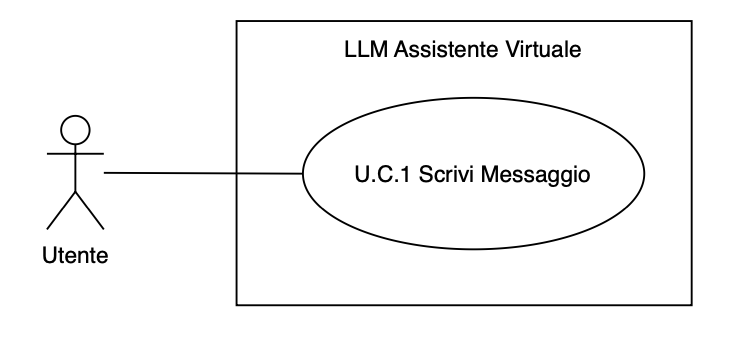
\includegraphics[width=0.7\textwidth]{img/UC1.png}
    \caption{U.C.1 Scrivi Messaggio}
\end{figure}
\newpage

\subsubsection{U.C.2 Visualizza Risposta}
\begin{itemize}
    \item \textbf{Attore}: Utente
    \item \textbf{Attore Secondario}: OpenAi
    \item \textbf{Precondizioni}:  L'utente ha inviato una domanda al bot e attende una risposta.
    \item \textbf{Postcondizioni}: Utente riceve una risposta dal bot coerente alla domanda che ha effettuato.
    \item \textbf{Scenario principale}:  Dopo aver inviato una domanda, l'utente attende la risposta elaborata dall’\href{https://code7crusaders.github.io/docs/RTB/documentazione_interna/glossario.html#llm-large-language-model}{\textit{LLM}\textsuperscript{G}} che viene visualizzata nella finestra della chat.
    \item \textbf{Generalizzazioni}: -
    \item \textbf{Estensioni}: U.C.2.1
    \item \textbf{Inclusione}: -
\end{itemize}
\begin{figure}[H]
    \centering
    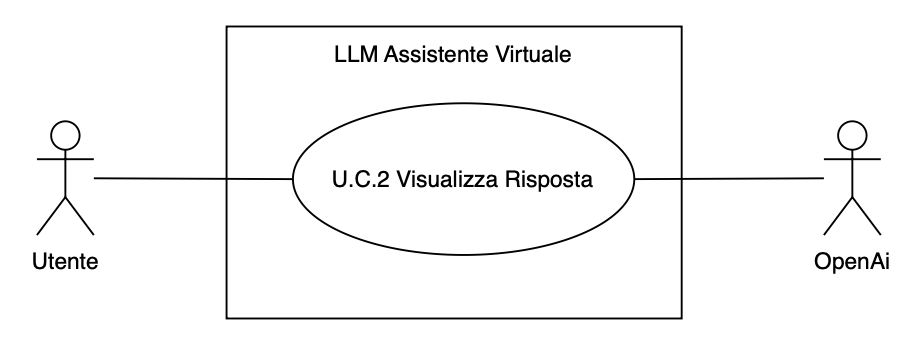
\includegraphics[width=0.8\textwidth]{img/UC2.png}
    \caption{U.C.2 Visualizza Risposta}
\end{figure}
\newpage

\subsubsection{U.C.2.1 Prodotto non trovato}
\begin{itemize}
    \item \textbf{Attore}: Utente
    \item \textbf{Precondizioni}: L'utente richiede informazioni su un prodotto non presente nel database del sistema.
    \item \textbf{Postcondizioni}: L'utente riceve una risposta da parte del \href{https://code7crusaders.github.io/docs/RTB/documentazione_interna/glossario.html#llm-large-language-model}{LLM\textsuperscript{G}}, non è possibile elaborare l'informazione.
    \item \textbf{Scenario principale}: L'utente invia una domanda su un prodotto specifico, il sistema cerca nel database ma non trova risultati. Un messaggio di errore avvisa l'utente che il prodotto 
    \item \textbf{Generalizzazioni}: -
    \item \textbf{Estensioni}: -
    \item \textbf{Inclusione}: -
\end{itemize}
\begin{figure}[H]
    \centering
    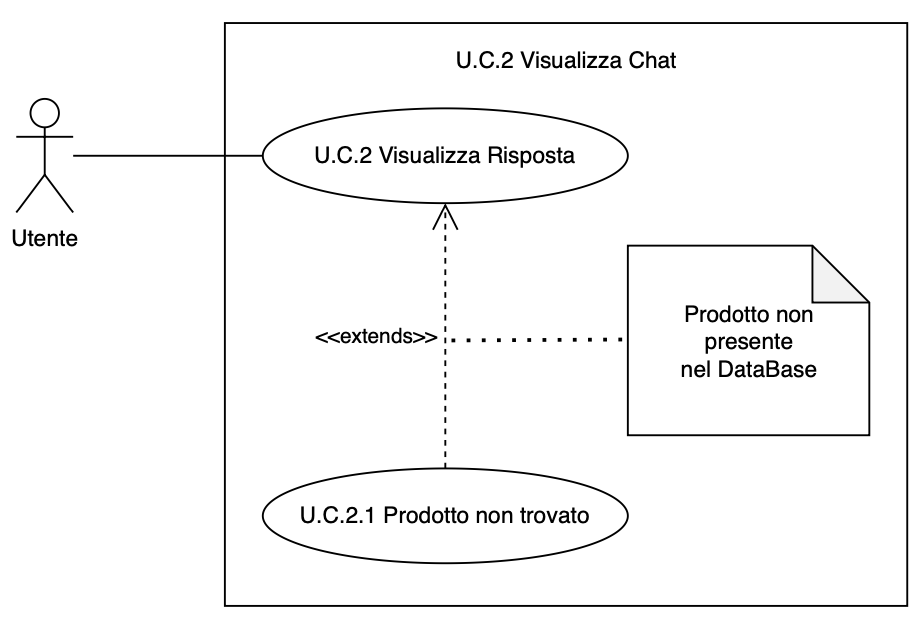
\includegraphics[width=0.7\textwidth]{img/UC2.1.png}
    \caption{U.C.2.1 Prodotto non Trovato}
\end{figure}
\newpage
 
\subsubsection{U.C.3 Seleziona Template}
\begin{itemize}
    \item \textbf{Attore}: Utente
    \item \textbf{Precondizioni}: L'utente ha effettuato l'accesso ed è nella chat. Vuole selezionare una domanda predefinita tra quelle suggerite dal sistema. 
    \item \textbf{Postcondizioni}: L'utente riceve una risposta templatizzata senza dover formulare una domanda manuale.(senza dover chiamare l’\href{https://code7crusaders.github.io/docs/RTB/documentazione_interna/glossario.html#llm-large-language-model}{\textit{LLM}\textsuperscript{G}}).
    \item \textbf{Scenario principale}: L'utente visualizza un elenco di domande suggerite, ne seleziona una e il sistema fornisce immediatamente una risposta.
    \item \textbf{Generalizzazioni}: -
    \item \textbf{Estensioni}: -
    \item \textbf{Inclusione}: -
\end{itemize}
\begin{figure}[H]
    \centering
    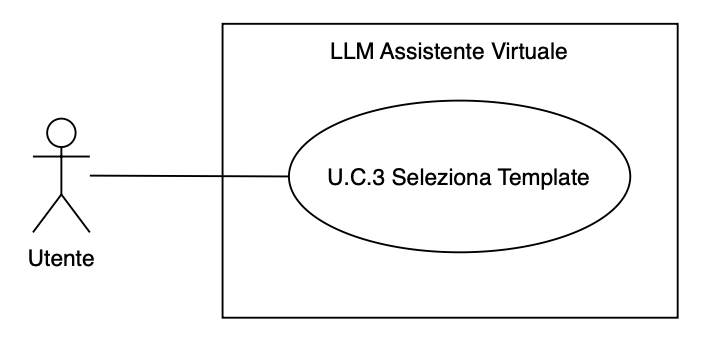
\includegraphics[width=0.7\textwidth]{img/UC3.png}
    \caption{U.C.3 Seleziona Template}
\end{figure}
\newpage

\subsubsection{U.C.4 Visualizza lista conversazioni precedenti}
\begin{itemize}
    \item \textbf{Attore}: Utente
    \item \textbf{Precondizioni}: L'utente ha effettuato l'accesso e in passato ha salvato almeno una conversazione.
    \item \textbf{Postcondizioni}: L'utente visualizza l'elenco delle conversazioni salvate.
    \item \textbf{Scenario principale}: L'utente accede alla sezione delle conversazioni e visualizza una lista ordinata delle sue conversazioni passate.
    \item \textbf{Generalizzazioni}: -
    \item \textbf{Estensioni}: -
    \item \textbf{Inclusione}: -
\end{itemize}
\begin{figure}[H]
    \centering
    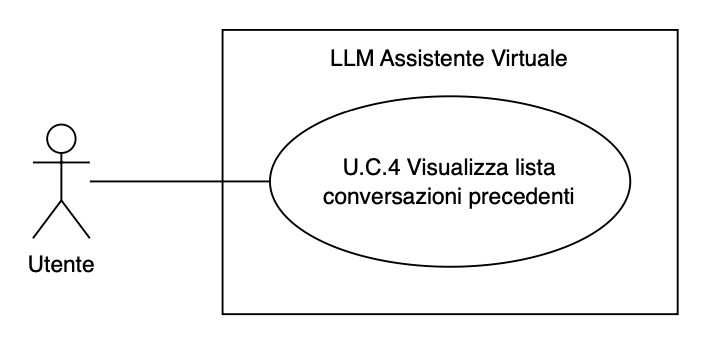
\includegraphics[width=0.7\textwidth]{img/UC4.png}
    \caption{U.C.4 Visualizza lista conversazioni precedenti}
\end{figure}
\newpage

\subsubsection{U.C.5 Visualizza Singola Conversazione Precedente}
\begin{itemize}
    \item \textbf{Attore}: Utente
    \item \textbf{Precondizioni}: L'utente ha effettuato l'accesso e in passato ha salvato almeno una conversazione.
    \item \textbf{Postcondizioni}: L'utente visualizza una conversazione salvata.
    \item \textbf{Scenario principale}: L'utente accede alla sezione delle conversazioni e visualizza una delle sue conversazioni passate.
    \item \textbf{Generalizzazioni}: -
    \item \textbf{Estensioni}: -
    \item \textbf{Inclusione}: -
\end{itemize}
\begin{figure}[H]
    \centering
    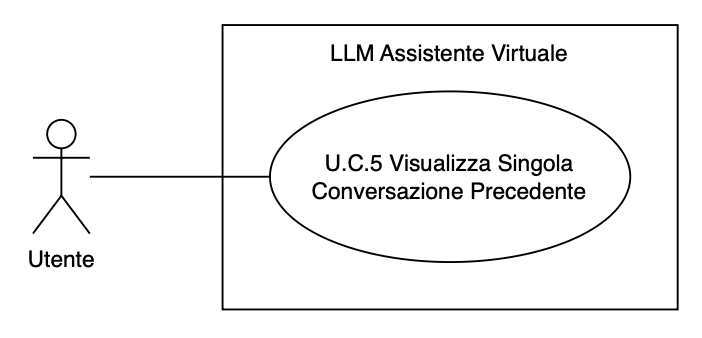
\includegraphics[width=0.7\textwidth]{img/UC5.png}
    \caption{U.C.5 Visualizza Singola Conversazione Precedente}
\end{figure}
\newpage

\subsubsection{U.C.6 Login}
\begin{itemize}
    \item \textbf{Attore}: Utente
    \item \textbf{Precondizioni}: L'utente è registrato e desidera accedere al sistema.
    \item \textbf{Postcondizioni}: L'utente accede con successo al sistema e può utilizzare le funzionalità disponibili.
    \item \textbf{Scenario principale}: L'utente inserisce il proprio username e password nei campi di accesso ed effettua l’accesso. Il sistema verifica le credenziali e consente l'accesso.  
    \item \textbf{Generalizzazioni}: -
    \item \textbf{Estensioni}: -
    \item \textbf{Inclusione}: U.C.6.1, U.C.6.2
\end{itemize}
\begin{figure}[H]
    \centering
    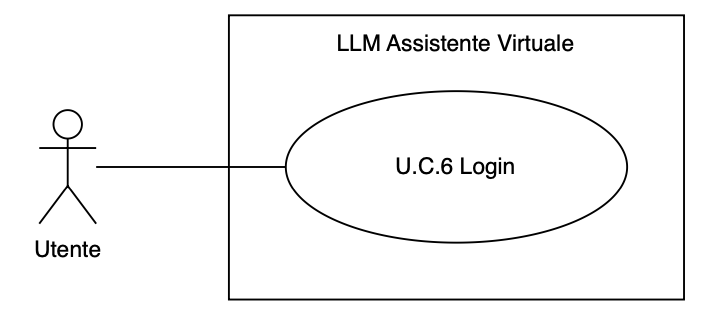
\includegraphics[width=0.7\textwidth]{img/UC6.png}
    \caption{U.C.6 Login}
\end{figure}
\newpage

\subsubsection{U.C.6.1 Inserisci Username}
\begin{itemize}
    \item \textbf{Attore}: Utente
    \item \textbf{Precondizioni}: L'utente desidera accedere al sistema.
    \item \textbf{Postcondizioni}: L'username è stato inserito correttamente nel campo corrispondente.
    \item \textbf{Scenario principale}: L'utente digita il proprio username nel campo di testo dedicato e procede con l'autenticazione.
    \item \textbf{Generalizzazioni}: -
    \item \textbf{Estensioni}: U.C.6.4, U.C.6.5
    \item \textbf{Inclusione}: -
\end{itemize}
\begin{figure}[H]
    \centering
    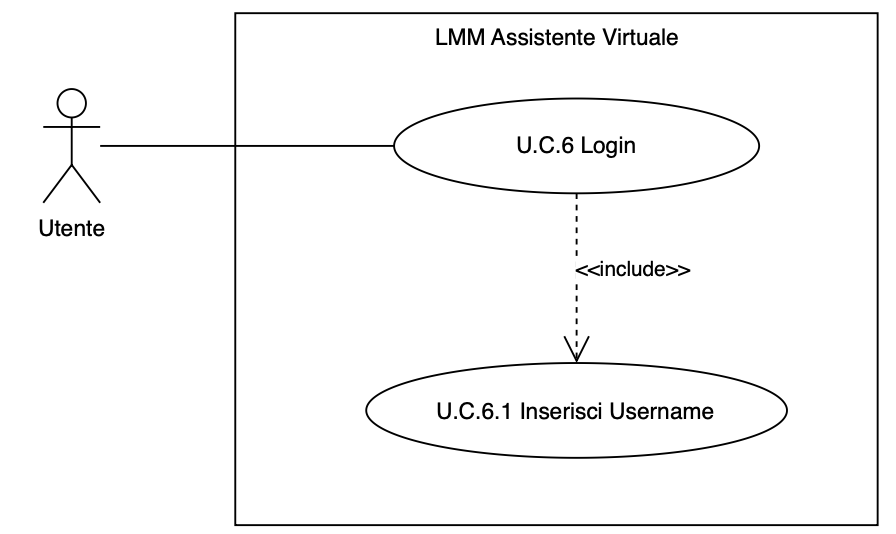
\includegraphics[width=0.8\textwidth]{img/UC6.1.png}
    \caption{U.C.6.1 Inserisci Username}
\end{figure}
\newpage

\subsubsection{U.C.6.2 Inserisci Password}
\begin{itemize}
    \item \textbf{Attore}: Utente
    \item \textbf{Precondizioni}: L'utente desidera accedere al sistema.
    \item \textbf{Postcondizioni}: La password è stata inserita correttamente nel campo corrispondente.
    \item \textbf{Scenario principale}: L'utente digita la password nel campo di testo e procede con l'autenticazione.
    \item \textbf{Generalizzazioni}: -
    \item \textbf{Estensioni}: U.C.6.3, U.C.6.5
    \item \textbf{Inclusione}: -
\end{itemize}
\begin{figure}[H]
    \centering
    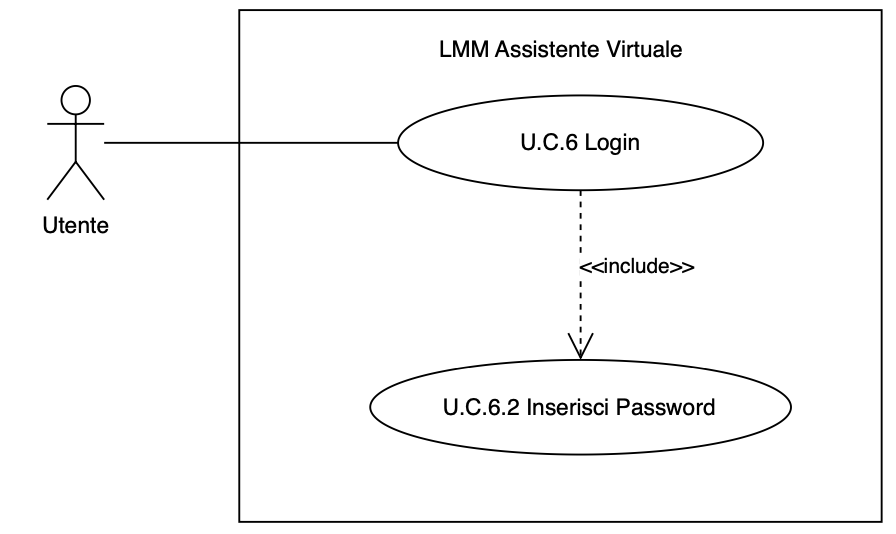
\includegraphics[width=0.8\textwidth]{img/UC6.2.png}
    \caption{U.C.6.2 Inserisci Password}
\end{figure}
\newpage

\subsubsection{U.C.6.3 Password Errata}
\begin{itemize}
    \item \textbf{Attore}: Utente
    \item \textbf{Precondizioni}: L'utente ha inserito una password non corrispondente a quella registrata.
    \item \textbf{Postcondizioni}: L'accesso viene negato e il sistema visualizza un messaggio di errore.
    \item \textbf{Scenario principale}: L'utente inserisce una password sbagliata. Il sistema verifica le credenziali, rileva l'errore e mostra un messaggio che informa l'utente dell'errore.
    \item \textbf{Generalizzazioni}: -
    \item \textbf{Estensioni}: -
    \item \textbf{Inclusione}: -
\end{itemize}
\begin{figure}[H]
    \centering
    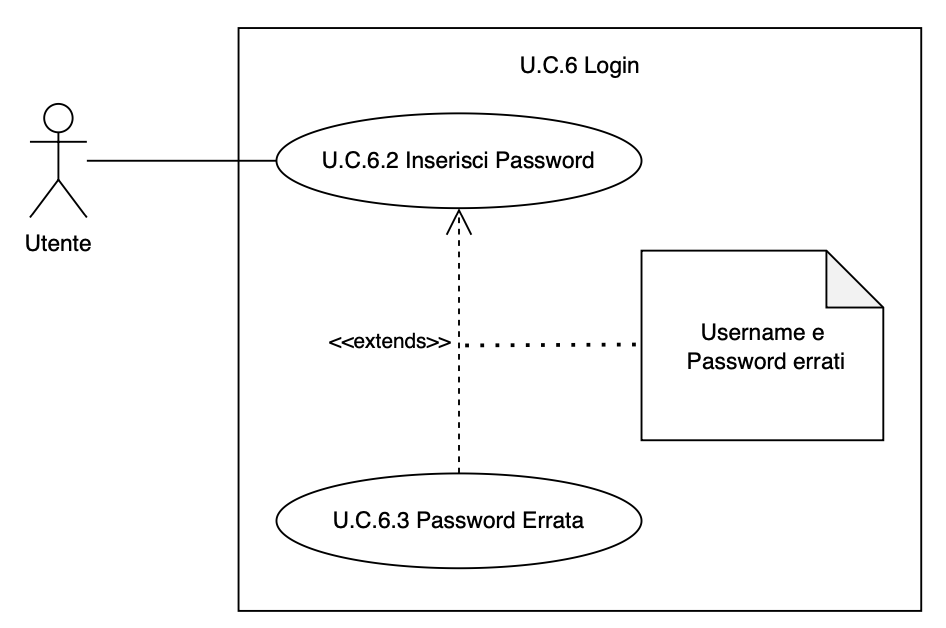
\includegraphics[width=0.8\textwidth]{img/UC6.3.png}
    \caption{U.C.6.3 Password Errata}
\end{figure}
\newpage

\subsubsection{U.C.6.4 Username Errato}
\begin{itemize}
    \item \textbf{Attore}: Utente
    \item \textbf{Precondizioni}: L'utente ha inserito un username non registrato o con errori di battitura.
    \item \textbf{Postcondizioni}: L'accesso viene negato e il sistema visualizza un messaggio di errore.
    \item \textbf{Scenario principale}: L'utente digita un username inesistente. Il sistema verifica i dati e notifica l'errore.
    \item \textbf{Generalizzazioni}: -
    \item \textbf{Estensioni}: -
    \item \textbf{Inclusione}: -
\end{itemize}
\begin{figure}[H]
    \centering
    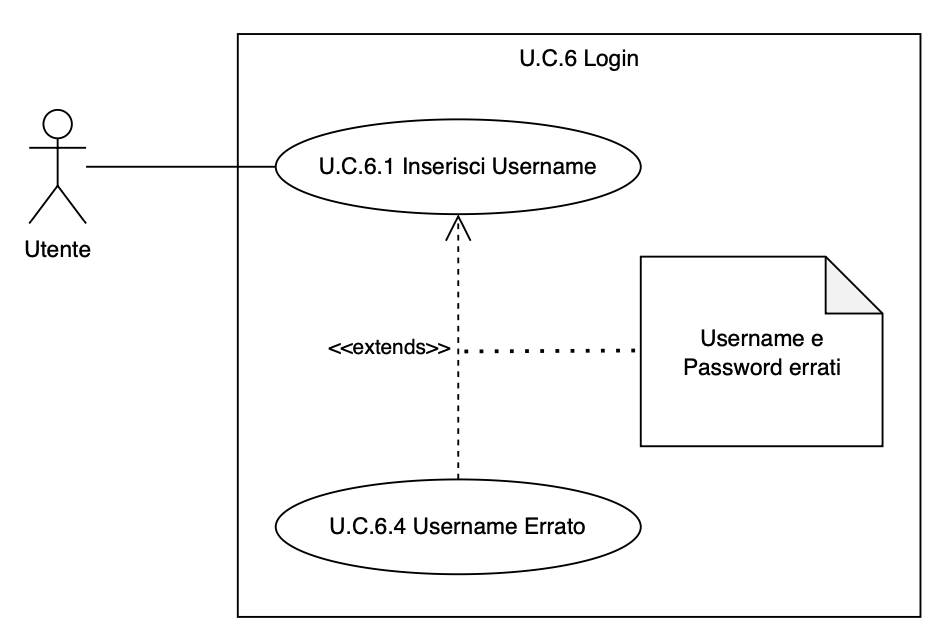
\includegraphics[width=0.8\textwidth]{img/UC6.4.png}
    \caption{U.C.6.4 Username Errato}
\end{figure}
\newpage

\subsubsection{U.C.6.5 Caratteri non Validi}
\begin{itemize}
    \item \textbf{Attore}: Utente
    \item \textbf{Precondizioni}: L'utente inserisce dati che contengono caratteri non ammessi.
    \item \textbf{Postcondizioni}: L'accesso viene negato e viene mostrato un messaggio di errore specifico.
    \item \textbf{Scenario principale}: L'accesso viene negato e viene mostrato un messaggio di errore specifico.
    \item \textbf{Generalizzazioni}: -
    \item \textbf{Estensioni}: -
    \item \textbf{Inclusione}: -
\end{itemize}
\begin{figure}[H]
    \centering
    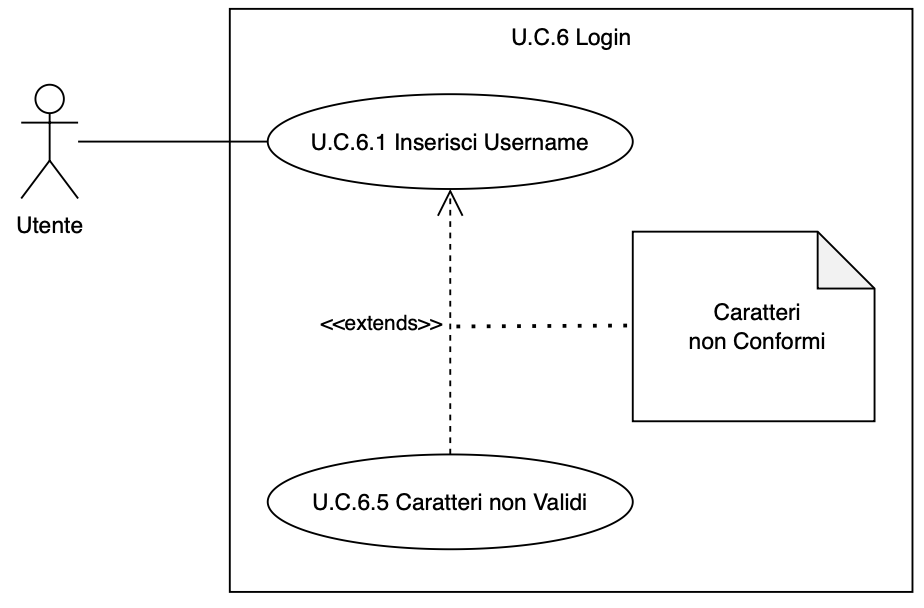
\includegraphics[width=0.6\textwidth]{img/UC6.5.1.png}
    %\caption{U.C.6.5 Caratteri non Validi}
\end{figure}
\begin{figure}[H]
    \centering
    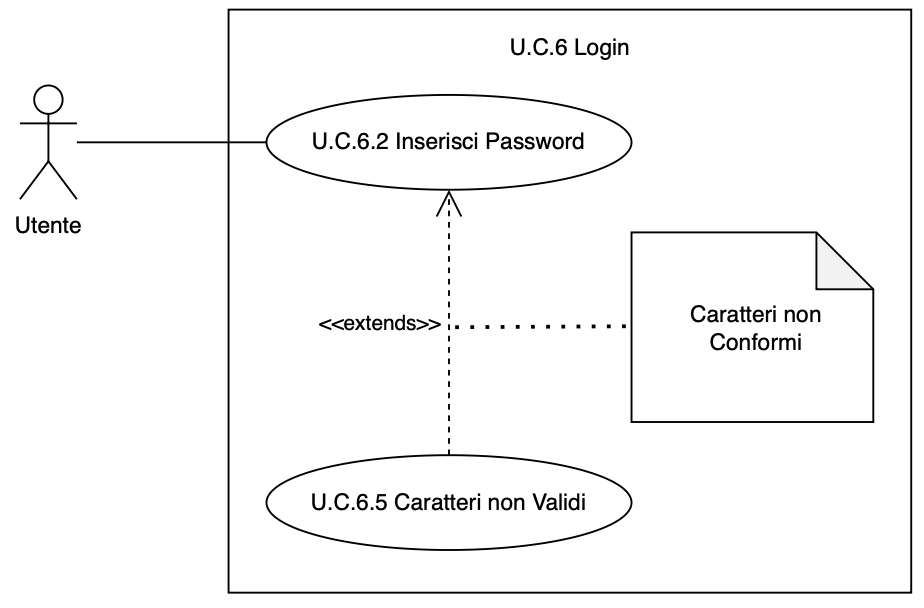
\includegraphics[width=0.6\textwidth]{img/UC6.5.2.png}
    \caption{U.C.6.5 Caratteri non Validi}
\end{figure}
\newpage

\subsubsection{U.C.7 Sign Up}
\begin{itemize}
    \item \textbf{Attore}: Utente
    \item \textbf{Precondizioni}: L'utente non è registrato al sistema e desidera accedere ai servizi.
    \item \textbf{Postcondizioni}: L'utente viene registrato con successo e può accedere al sistema.
    \item \textbf{Scenario principale}: L'utente seleziona l'opzione di registrazione, compila i campi richiesti come username e password, e conferma l'operazione. Il sistema verifica i dati e completa la registrazione.
    \item \textbf{Generalizzazioni}: -
    \item \textbf{Estensioni}: -
    \item \textbf{Inclusione}: U.C.7.1, U.C.7.2
\end{itemize}
\begin{figure}[H]
    \centering
    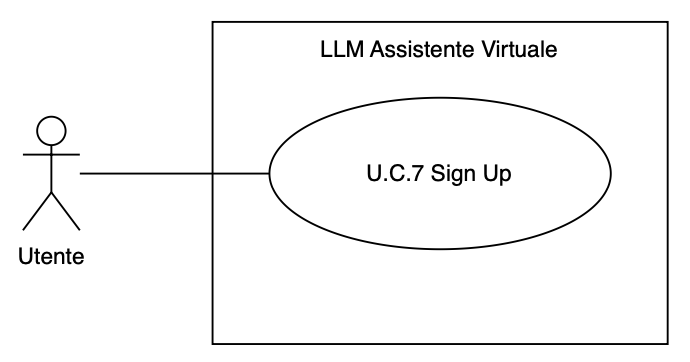
\includegraphics[width=0.7\textwidth]{img/UC7.png}
    \caption{U.C.7 Sign Up}
\end{figure}
\newpage

\subsubsection{U.C.7.1 Inserisci Username}
\begin{itemize}
    \item \textbf{Attore}: Utente
    \item \textbf{Precondizioni}: L'utente non è registrato e sta procedendo alla creazione di un account.
    \item \textbf{Postcondizioni}: L'username è stato inserito correttamente nel sistema.
    \item \textbf{Scenario principale}: L'utente compila il campo "Username" durante la registrazione e procede al passaggio successivo.
    \item \textbf{Generalizzazioni}: -
    \item \textbf{Estensioni}: -
    \item \textbf{Inclusione}: U.C.7.3, U.C.7.4, U.C.7.6
\end{itemize}
\begin{figure}[H]
    \centering
    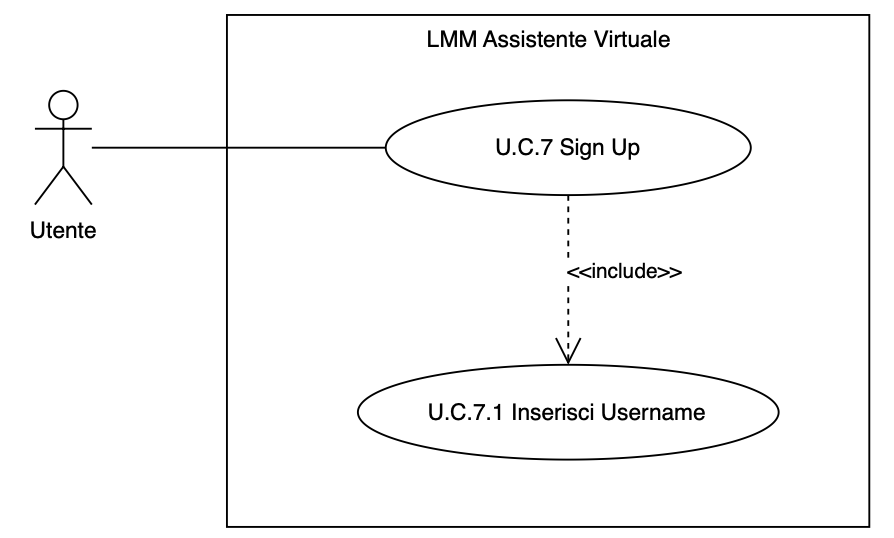
\includegraphics[width=0.8\textwidth]{img/UC7.1.png}
    \caption{U.C.7.1 Inserisci Username}
\end{figure}
\newpage

\subsubsection{U.C.7.2 Inserisci Password}
\begin{itemize}
    \item \textbf{Attore}: Utente
    \item \textbf{Precondizioni}: L'utente non è registrato e sta completando il processo di registrazione.
    \item \textbf{Postcondizioni}: La password viene salvata correttamente nel sistema.
    \item \textbf{Scenario principale}: L'utente inserisce una password nel campo corrispondente e procede con la registrazione. 
    \item \textbf{Generalizzazioni}: -
    \item \textbf{Estensioni}: -
    \item \textbf{Inclusione}: U.C.7.3, U.C.7.5
\end{itemize}
\begin{figure}[H]
    \centering
    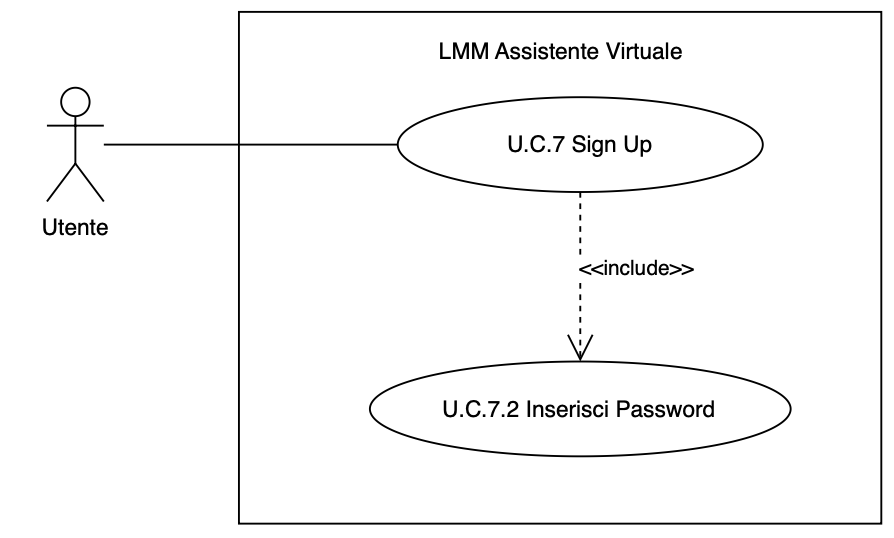
\includegraphics[width=0.8\textwidth]{img/UC7.2.png}
    \caption{U.C.7.2 Inserisci Password}
\end{figure}
\newpage

\subsubsection{U.C.7.3 Caratteri non Validi}
\begin{itemize}
    \item \textbf{Attore}: Utente
    \item \textbf{Precondizioni}: Durante la registrazione, l'utente inserisce caratteri non consentiti nel campo username o password.
    \item \textbf{Postcondizioni}: La registrazione viene interrotta e l'utente riceve un messaggio di errore.
    \item \textbf{Scenario principale}: L'utente tenta di registrarsi ma utilizza caratteri non validi nei campi obbligatori. Il sistema rileva l'errore e avvisa l'utente.
    \item \textbf{Generalizzazioni}: -
    \item \textbf{Estensioni}: -
    \item \textbf{Inclusione}: -
\end{itemize}
\begin{figure}[H]
    \centering
    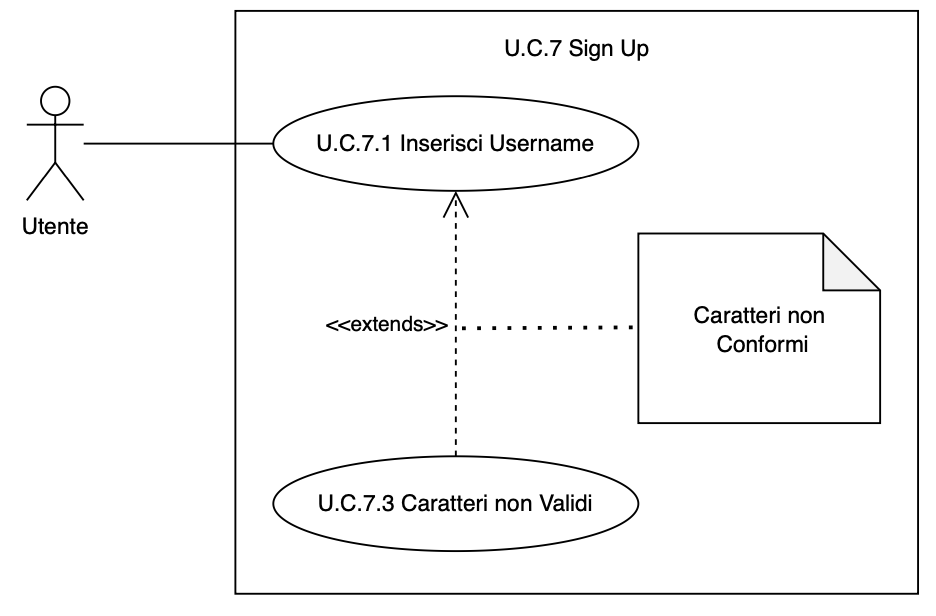
\includegraphics[width=0.6\textwidth]{img/UC7.3.1.png}
    %\caption{U.C.7.3 Caratteri non Validi}
\end{figure}
\begin{figure}[H]
    \centering
    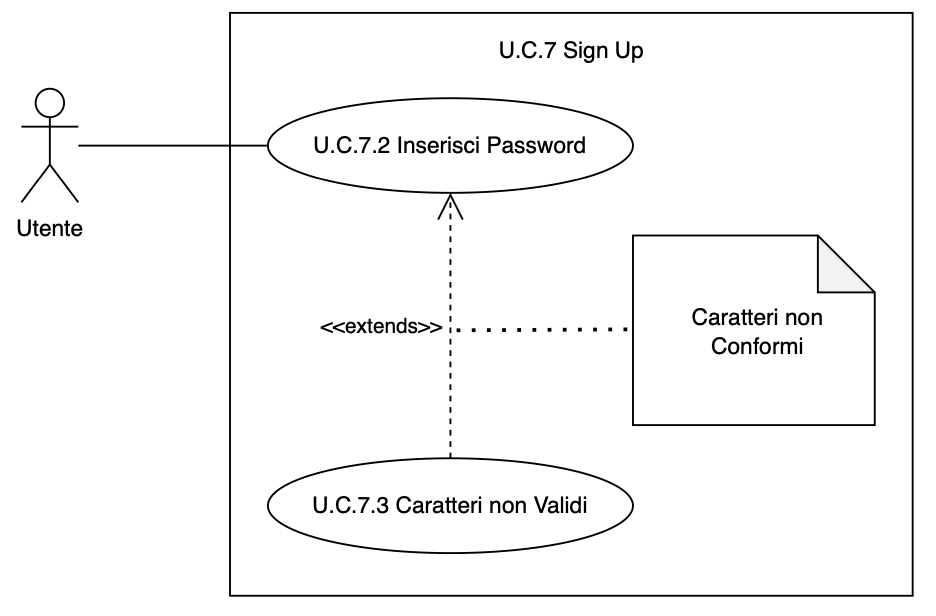
\includegraphics[width=0.6\textwidth]{img/UC7.3.2.png}
    \caption{U.C.7.3 Caratteri non Validi}
\end{figure}
\newpage

\subsubsection{U.C.7.4 Username troppo Lungo}
\begin{itemize}
    \item \textbf{Attore}: Utente
    \item \textbf{Precondizioni}: L'utente inserisce un username che supera il limite massimo di caratteri consentiti.
    \item \textbf{Postcondizioni}: La registrazione non viene completata e l'utente riceve un messaggio di errore. 
    \item \textbf{Scenario principale}: Durante la registrazione, il sistema rileva che l'username è troppo lungo e informa l'utente. 
    \item \textbf{Generalizzazioni}: -
    \item \textbf{Estensioni}: -
    \item \textbf{Inclusione}: -
\end{itemize}
\begin{figure}[H]
    \centering
    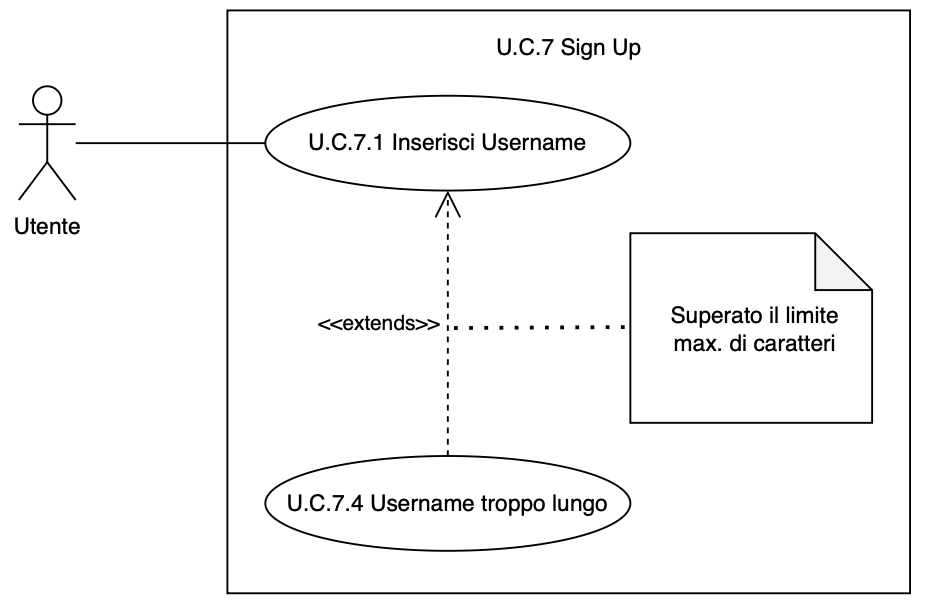
\includegraphics[width=0.8\textwidth]{img/UC7.4.png}
    \caption{U.C.7.4 Username troppo Lungo}
\end{figure}
\newpage

\subsubsection{U.C.7.5 Password troppo Lunga}
\begin{itemize}
    \item \textbf{Attore}: Utente
    \item \textbf{Precondizioni}: L'utente inserisce una password che supera il limite massimo consentito.
    \item \textbf{Postcondizioni}: La registrazione viene bloccata e l'utente viene informato dell'errore.  
    \item \textbf{Scenario principale}: L'utente tenta di completare la registrazione ma il sistema respinge la password perché troppo lunga. 
    \item \textbf{Generalizzazioni}: -
    \item \textbf{Estensioni}: -
    \item \textbf{Inclusione}: -
\end{itemize}
\begin{figure}[H]
    \centering
    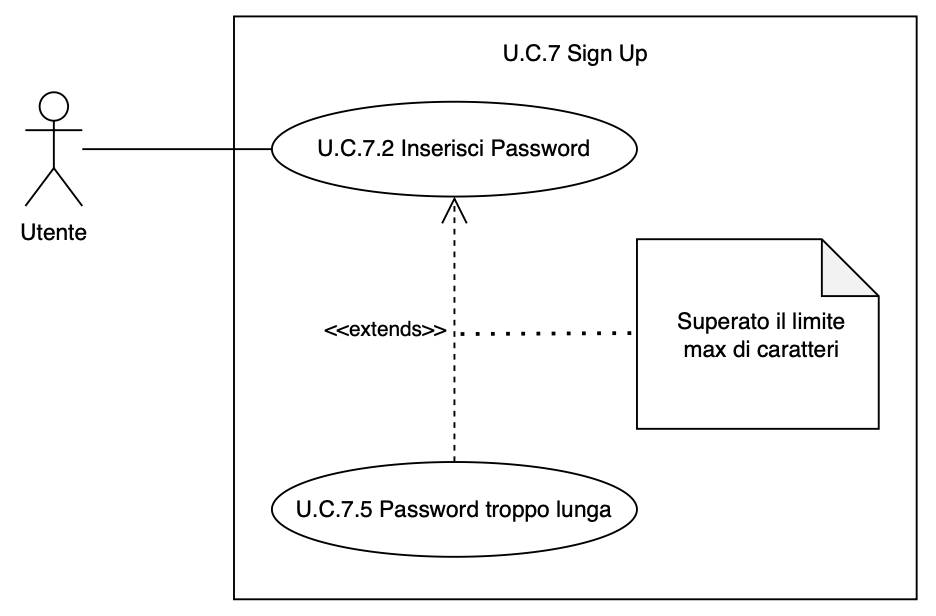
\includegraphics[width=0.8\textwidth]{img/UC7.5.png}
    \caption{U.C.7.5 Password troppo lunga}
\end{figure}
\newpage

\subsubsection{U.C.7.6 Username già presente}
\begin{itemize}
    \item \textbf{Attore}: Utente
    \item \textbf{Precondizioni}: L'utente inserisce un username già esistente nel sistema.
    \item \textbf{Postcondizioni}: La registrazione viene interrotta e il sistema suggerisce di scegliere un altro username.  
    \item \textbf{Scenario principale}: L'utente tenta di registrarsi con uno username già utilizzato e il sistema blocca l'operazione con un messaggio informativo. 
    \item \textbf{Generalizzazioni}: -
    \item \textbf{Estensioni}: -
    \item \textbf{Inclusione}: -
\end{itemize}
\begin{figure}[H]
    \centering
    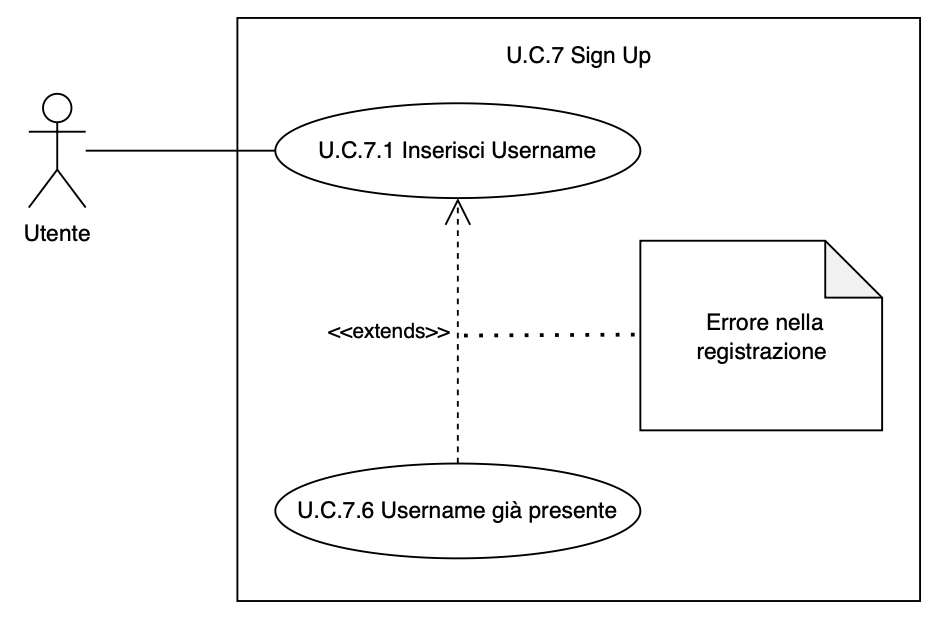
\includegraphics[width=0.8\textwidth]{img/UC7.6.png}
    \caption{U.C.7.6 Username già presente}
\end{figure}
\newpage

\subsubsection{U.C.8 Salva Chat}
\begin{itemize}
    \item \textbf{Attore}: Utente
    \item \textbf{Precondizioni}: L'utente ha completato una conversazione con il bot e desidera conservarlo per consultazioni future. 
    \item \textbf{Postcondizioni}: La conversazione viene salvata e aggiunta all'elenco delle chat salvate.
    \item \textbf{Scenario principale}: Dopo aver terminato la conversazione, l'utente seleziona l'opzione "Salva Chat" e il sistema archivia la conversazione.
    \item \textbf{Generalizzazioni}: -
    \item \textbf{Estensioni}: U.C.8.1
    \item \textbf{Inclusione}: -
\end{itemize}
\begin{figure}[H]
    \centering
    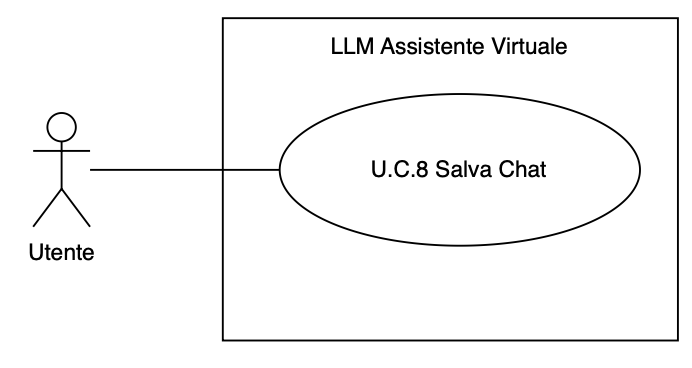
\includegraphics[width=0.7\textwidth]{img/UC8.png}
    \caption{U.C.8 Salva Chat}
\end{figure}
\newpage

\subsubsection{U.C.8.1 Memoria Piena}
\begin{itemize}
    \item \textbf{Attore}: Utente
    \item \textbf{Precondizioni}: L'utente ha superato il limite di conversazioni salvabili nel proprio account.
    \item \textbf{Postcondizioni}: La conversazione non viene salvata e l'utente riceve un avviso.
    \item \textbf{Scenario principale}: L'utente tenta di salvare una chat, ma il sistema rileva che lo spazio dedicato alle conversazioni è esaurito. Il sistema invita l'utente a eliminare alcune chat per liberare spazio.
    \item \textbf{Generalizzazioni}: -
    \item \textbf{Estensioni}: -
    \item \textbf{Inclusione}: -
\end{itemize}
\begin{figure}[H]
    \centering
    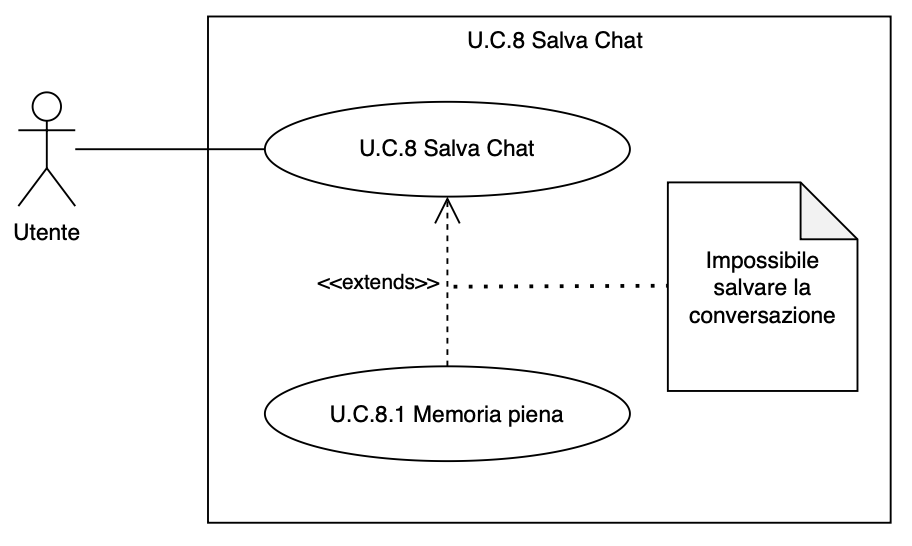
\includegraphics[width=0.8\textwidth]{img/UC8.1.png}
    \caption{U.C.8.1 Memoria Piena}
\end{figure}
\newpage

\subsubsection{U.C.9 Feedback Chat}
\begin{itemize}
    \item \textbf{Attore}: Utente
    \item \textbf{Precondizioni}: L'utente ha completato una conversazione con il bot e vuole esprimere un giudizio sulla qualità delle risposte ricevute.
    \item \textbf{Postcondizioni}: Il feedback viene registrato nel sistema per analisi future.
    \item \textbf{Scenario principale}: Dopo la conversazione, l'utente valuta il bot scegliendo un'opzione di feedback (positivo o negativo). Il sistema registra il giudizio per migliorare le prestazioni future.
    \item \textbf{Generalizzazioni}: -
    \item \textbf{Estensioni}: -
    \item \textbf{Inclusione}: -
\end{itemize}
\begin{figure}[H]
    \centering
    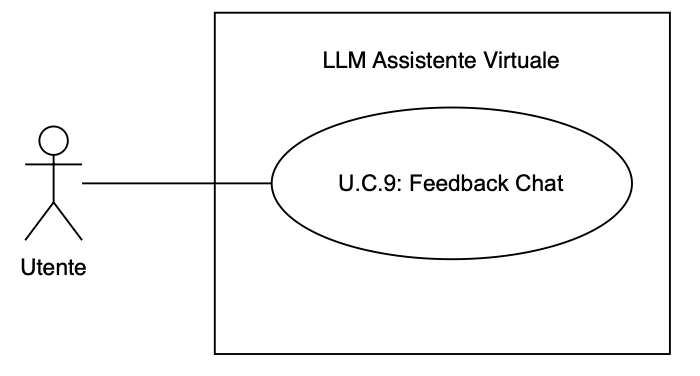
\includegraphics[width=0.7\textwidth]{img/UC9.png}
    \caption{U.C.9 Feedback Chat}
\end{figure}
\newpage

\subsubsection{U.C.10: Creazione di un nuovo template}
\begin{itemize}
    \item \textbf{Attore}: Admin
    \item \textbf{Precondizioni}: L'amministratore ha effettuato l'accesso al sistema di gestione e ha selezionato l'opzione per creare un nuovo \href{https://code7crusaders.github.io/docs/RTB/documentazione_interna/glossario.html#template}{template\textsuperscript{G}}.
    \item \textbf{Postcondizioni}: Un nuovo \href{https://code7crusaders.github.io/docs/RTB/documentazione_interna/glossario.html#template}{template\textsuperscript{G}} con una domanda predefinita e una risposta associata è stato salvato nel sistema.
    \item \textbf{Scenario principale}: L'amministratore accede alla funzione di creazione di un nuovo \href{https://code7crusaders.github.io/docs/RTB/documentazione_interna/glossario.html#template}{template\textsuperscript{G}}. In questa sezione, inserisce una domanda predefinita e una risposta predefinita. Dopo aver verificato che i dati inseriti siano corretti, l'amministratore salva il nuovo \href{https://code7crusaders.github.io/docs/RTB/documentazione_interna/glossario.html#template}{template\textsuperscript{G}}, che diventa immediatamente disponibile per essere utilizzato dagli utenti nella chat.
    \item \textbf{Generalizzazioni}: -
    \item \textbf{Estensioni}: U.C.13
    \item \textbf{Inclusione}: -
\end{itemize}
\begin{figure}[H]
    \centering
    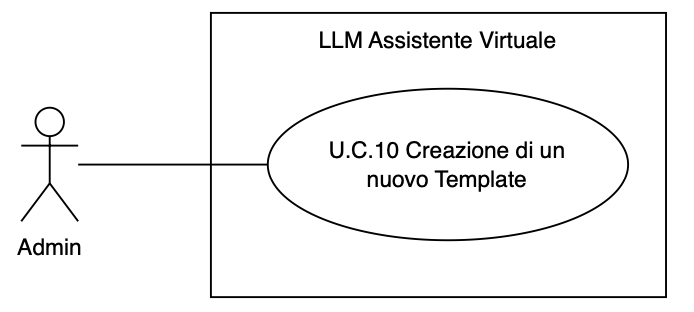
\includegraphics[width=0.7\textwidth]{img/UC10.png}
    \caption{U.C.10: Creazione di un nuovo template}
\end{figure}
\newpage

\subsubsection{U.C.11: Modifica di un template esistente}
\begin{itemize}
    \item \textbf{Attore}: Admin
    \item \textbf{Precondizioni}: L'amministratore ha effettuato l'accesso e ha selezionato un \href{https://code7crusaders.github.io/docs/RTB/documentazione_interna/glossario.html#template}{template\textsuperscript{G}} esistente dalla lista.
    \item \textbf{Postcondizioni}: Il \href{https://code7crusaders.github.io/docs/RTB/documentazione_interna/glossario.html#template}{template\textsuperscript{G}} selezionato viene aggiornato con i nuovi dati forniti.
    \item \textbf{Scenario principale}: L'amministratore visualizza l'elenco dei \href{https://code7crusaders.github.io/docs/RTB/documentazione_interna/glossario.html#template}{template\textsuperscript{G}} disponibili e seleziona quello che desidera modificare. Accede quindi ai dettagli del \href{https://code7crusaders.github.io/docs/RTB/documentazione_interna/glossario.html#template}{template\textsuperscript{G}}, dove può modificare sia la domanda predefinita che la risposta associata. Dopo aver apportato le modifiche necessarie, l'amministratore salva i cambiamenti, aggiornando così il \href{https://code7crusaders.github.io/docs/RTB/documentazione_interna/glossario.html#template}{template\textsuperscript{G}} nel sistema. Le modifiche apportate sono immediatamente visibili agli utenti quando utilizzano la funzione di selezione delle domande predefinite. 
    \item \textbf{Generalizzazioni}: -
    \item \textbf{Estensioni}: U.C.13
    \item \textbf{Inclusione}: -
\end{itemize}
\begin{figure}[H]
    \centering
    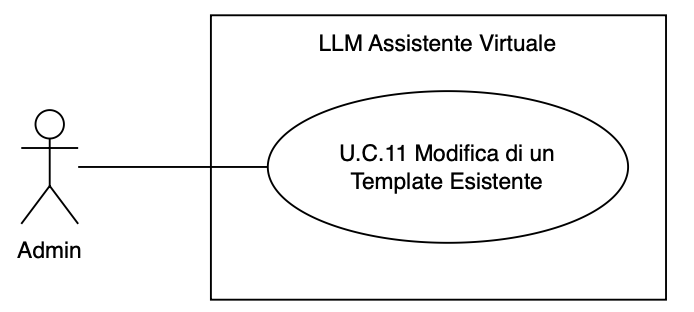
\includegraphics[width=0.7\textwidth]{img/UC11.png}
    \caption{U.C.11: Modifica di un template esistente}
\end{figure}
\newpage

\subsubsection{U.C.12: Elimina un template esistente}
\begin{itemize}
    \item \textbf{Attore}: Admin
    \item \textbf{Precondizioni}: L'amministratore ha effettuato l'accesso e ha selezionato un \href{https://code7crusaders.github.io/docs/RTB/documentazione_interna/glossario.html#template}{template\textsuperscript{G}} esistente dalla lista. 
    \item \textbf{Postcondizioni}: Il \href{https://code7crusaders.github.io/docs/RTB/documentazione_interna/glossario.html#template}{template\textsuperscript{G}} viene eliminato dal sistema e non è più disponibile per gli utenti.
    \item \textbf{Scenario principale}: L'amministratore, dalla lista dei \href{https://code7crusaders.github.io/docs/RTB/documentazione_interna/glossario.html#template}{template\textsuperscript{G}}, individua quello che intende eliminare. Dopo aver selezionato il \href{https://code7crusaders.github.io/docs/RTB/documentazione_interna/glossario.html#template}{template\textsuperscript{G}}, conferma l'operazione tramite un'apposita finestra di dialogo. Il sistema procede quindi a rimuovere il \href{https://code7crusaders.github.io/docs/RTB/documentazione_interna/glossario.html#template}{template\textsuperscript{G}}, aggiornando l'elenco dei \href{https://code7crusaders.github.io/docs/RTB/documentazione_interna/glossario.html#template}{template\textsuperscript{G}} disponibili. Da quel momento, la domanda predefinita associata non sarà più accessibile agli utenti.
    \item \textbf{Generalizzazioni}: -
    \item \textbf{Estensioni}: -
    \item \textbf{Inclusione}: -
\end{itemize}
\begin{figure}[H]
    \centering
    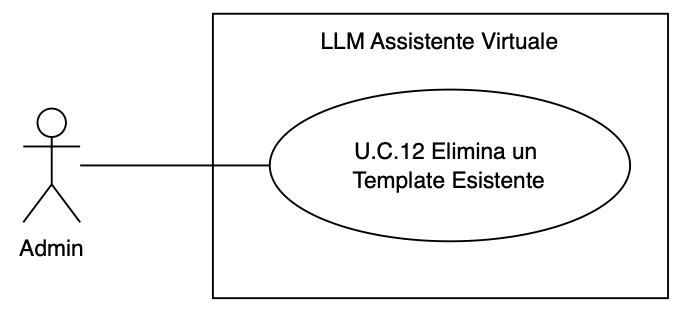
\includegraphics[width=0.7\textwidth]{img/UC12.png}
    \caption{U.C.12: Elimina un template esistente}
\end{figure}
\newpage

\subsubsection{U.C.13 Controllo Validità Formato}
\begin{itemize}
    \item \textbf{Attore}: Admin
    \item \textbf{Precondizioni}: L'amministratore sta creando o modificando un \href{https://code7crusaders.github.io/docs/RTB/documentazione_interna/glossario.html#template}{template\textsuperscript{G}}, ma inserisce un formato non valido (ad esempio, una domanda vuota o una risposta eccessivamente lunga ecc..)
    \item \textbf{Postcondizioni}: Il sistema non consente di salvare il \href{https://code7crusaders.github.io/docs/RTB/documentazione_interna/glossario.html#template}{template\textsuperscript{G}} e informa l'amministratore dell'errore.
    \item \textbf{Scenario principale}: Durante la creazione o modifica di un \href{https://code7crusaders.github.io/docs/RTB/documentazione_interna/glossario.html#template}{template\textsuperscript{G}}, l'amministratore inserisce dati non conformi, come una domanda lasciata vuota o una risposta con caratteri non consentiti. Il sistema esegue un controllo sui dati inseriti e rileva l'errore, bloccando il salvataggio del \href{https://code7crusaders.github.io/docs/RTB/documentazione_interna/glossario.html#template}{template\textsuperscript{G}}. Viene visualizzato un messaggio di errore chiaro che spiega il problema e invita l'amministratore a correggere i dati prima di procedere con il salvataggio.
    \item \textbf{Generalizzazioni}: -
    \item \textbf{Estensioni}: -
    \item \textbf{Inclusione}: -
\end{itemize}
\begin{figure}[H]
    \centering
    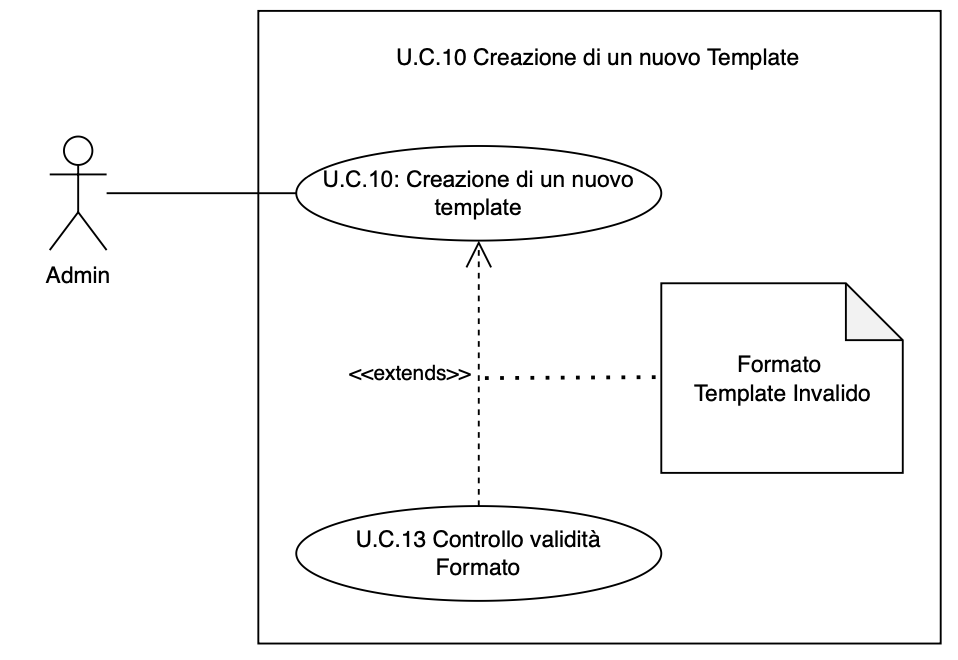
\includegraphics[width=0.6\textwidth]{img/UC13.1.png}
    %\caption{U.C.13 Controllo Validità Formato}
\end{figure}
\begin{figure}[H]
    \centering
    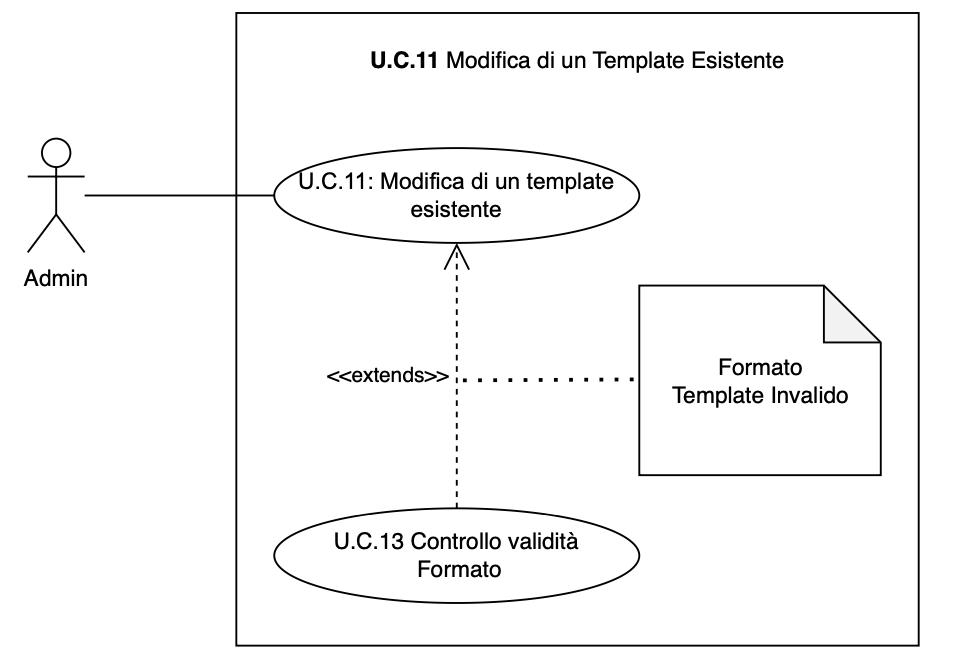
\includegraphics[width=0.6\textwidth]{img/UC13.2.png}
    \caption{U.C.13 Controllo Validità Formato}
\end{figure}
\newpage

\subsubsection{U.C.14: Visualizzazione delle metriche generali}
\begin{itemize}
    \item \textbf{Attore}: Admin
    \item \textbf{Precondizioni}: L'amministratore ha effettuato l'accesso alla dashboard di monitoraggio.
    \item \textbf{Postcondizioni}: L'amministratore visualizza le metriche principali del sistema.
    \item \textbf{Scenario principale}: L'amministratore seleziona l'opzione per visualizzare le statistiche generali e consulta i dati per analizzare le prestazioni del sistema.
    \item \textbf{Generalizzazioni}: -
    \item \textbf{Estensioni}: -
    \item \textbf{Inclusione}: -
\end{itemize}
\begin{figure}[H]
    \centering
    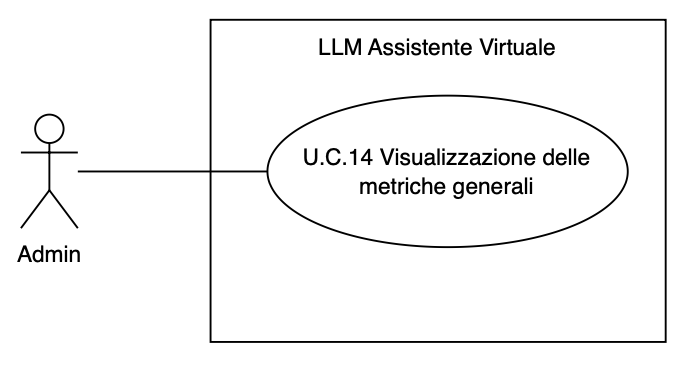
\includegraphics[width=0.7\textwidth]{img/UC14.png}
    \caption{U.C.14: Visualizzazione delle metriche generali}
\end{figure}
\newpage

\subsubsection{U.C.15: Visualizzazione Feedback Utenti}
\begin{itemize}
    \item \textbf{Attore}: Admin
    \item \textbf{Precondizioni}: L'amministratore ha effettuato l'accesso e ha selezionato la sezione relativa ai feedback degli utenti.
    \item \textbf{Postcondizioni}: I feedback degli utenti sulle risposte del chatbot sono stati visualizzati e analizzati.
    \item \textbf{Scenario principale}:  L'amministratore accede alla sezione dei feedback, consulta i giudizi degli utenti e utilizza le informazioni per migliorare il sistema.
    \item \textbf{Generalizzazioni}: -
    \item \textbf{Estensioni}: -
    \item \textbf{Inclusione}: -
\end{itemize}
\begin{figure}[H]
    \centering
    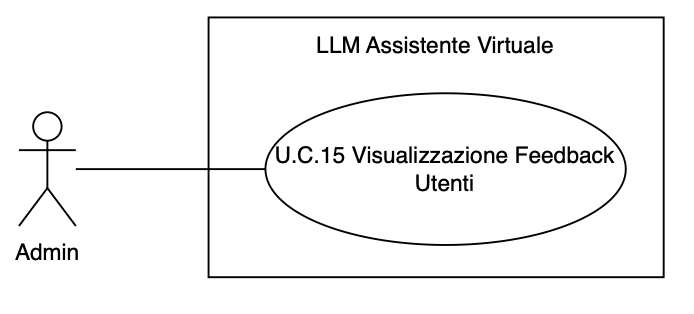
\includegraphics[width=0.7\textwidth]{img/UC15.png}
    \caption{U.C.15: Visualizzazione Feedback Utenti}
\end{figure}
\newpage

\subsubsection{U.C.16: Importazione di Dati}
\begin{itemize}
    \item \textbf{Attore}: Admin
    \item \textbf{Attore Secondario}: OpenAi
    \item \textbf{Precondizioni}: L'amministratore ha selezionato un file di dati da importare.
    \item \textbf{Postcondizioni}: I dati vengono caricati per la validazione.
    \item \textbf{Scenario principale}: L'amministratore seleziona il file dal proprio dispositivo e avvia il processo di importazione. Il sistema prepara i dati per la validazione.
    \item \textbf{Generalizzazioni}: -
    \item \textbf{Estensioni}: U.C.16.1
    \item \textbf{Inclusione}: -
\end{itemize}
\begin{figure}[H]
    \centering
    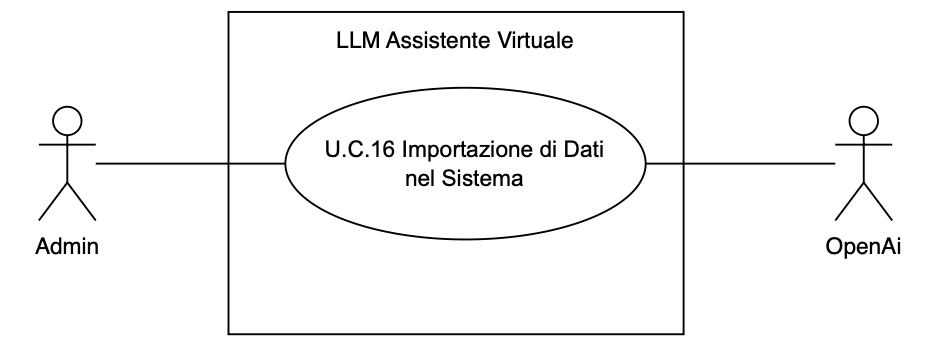
\includegraphics[width=0.8\textwidth]{img/UC16.png}
    \caption{U.C.16: Importazione di Dati}
\end{figure}
\newpage

\subsubsection{U.C.16.1: Validazione Formato}
\begin{itemize}
    \item \textbf{Attore}: Admin
    \item \textbf{Precondizioni}: L’amministratore vuole caricare un file dati da caricare.
    \item \textbf{Postcondizioni}: I file vengono respinti se il formato dati è sbagliato, altrimenti vengono importati.
    \item \textbf{Scenario principale}: Il sistema analizza il file, controlla la coerenza e il formato dei dati, se incoerente respinge e segnala errore.
    \item \textbf{Generalizzazioni}: -
    \item \textbf{Estensioni}: -
    \item \textbf{Inclusione}: -
\end{itemize}
\begin{figure}[H]
    \centering
    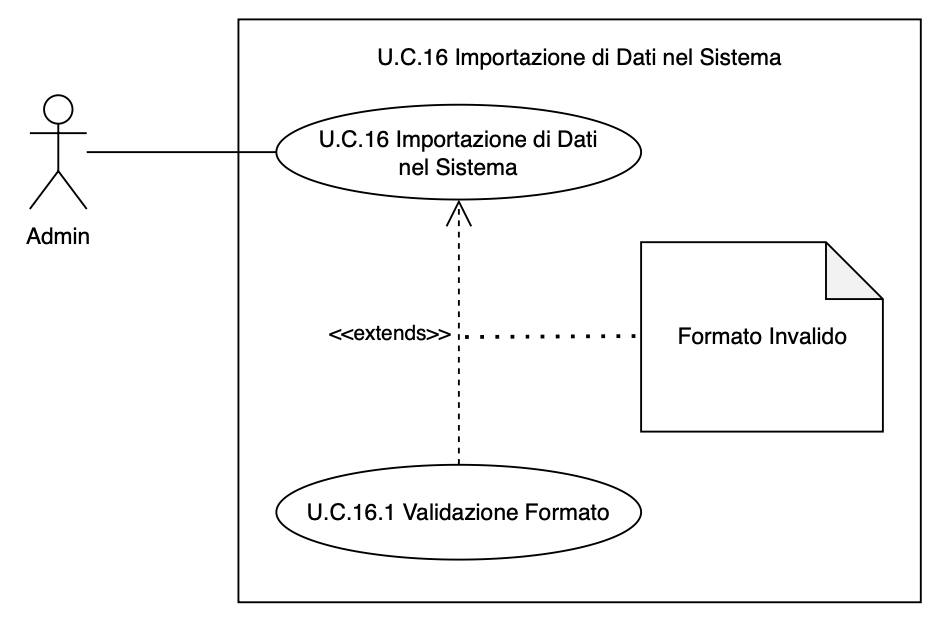
\includegraphics[width=0.7\textwidth]{img/UC16.1.png}
    \caption{U.C.16.1: Validazione Formato}
\end{figure}
\newpage

\subsubsection{U.C.17 Esportazione di Dati nel Sistema}
\begin{itemize}
    \item \textbf{Attore}: Admin
    \item \textbf{Precondizioni}: L’amministratore vuole esportare un file dati.
    \item \textbf{Postcondizioni}: I dati vengono esportati.
    \item \textbf{Scenario principale}: L'amministratore seleziona il file del database e avvia il processo di esportazione.
    \item \textbf{Generalizzazioni}: -
    \item \textbf{Estensioni}: -
    \item \textbf{Inclusione}: -
\end{itemize}
\begin{figure}[H]
    \centering
    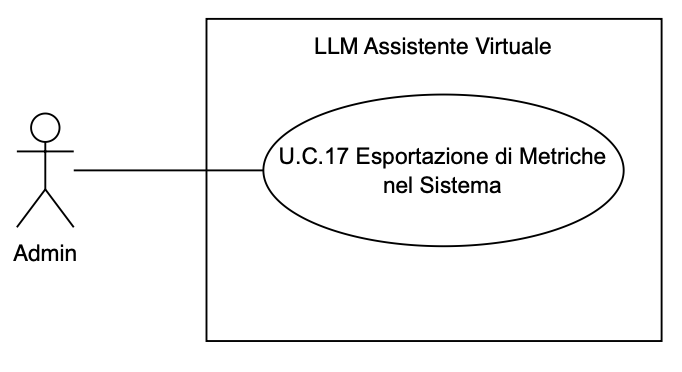
\includegraphics[width=0.7\textwidth]{img/UC17.png}
    \caption{U.C.17 Esportazione di Dati nel Sistema}
\end{figure}
\newpage

\subsubsection{U.C.18 Elimina Chat}
\begin{itemize}
    \item \textbf{Attore}: Utente
    \item \textbf{Precondizioni}: L'utente ha effettuato l'accesso ed è presente almeno una conversazione salvata.
    \item \textbf{Postcondizioni}: La conversazione selezionata viene eliminata dal sistema.
    \item \textbf{Scenario principale}: L'utente accede all'elenco delle chat salvate, seleziona una conversazione specifica e conferma l'eliminazione.
    \item \textbf{Generalizzazioni}: -
    \item \textbf{Estensioni}: -
    \item \textbf{Inclusione}: -
\end{itemize}
\begin{figure}[H]
    \centering
    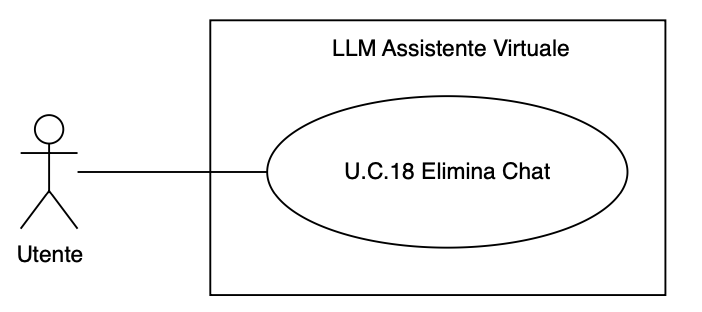
\includegraphics[width=0.7\textwidth]{img/UC18.png}
    \caption{U.C.18 Elimina Chat}
\end{figure}
\newpage

\subsubsection{U.C.19: Riprendi Conversazione}
\begin{itemize}
    \item \textbf{Attore}: Utente
    \item \textbf{Precondizioni}: L’utente ha effettuato l’accesso al sistema ed effettuato una conversazione
    \item \textbf{Postcondizioni}: L’utente riprende la conversazione con l’assistente virtuale.
    \item \textbf{Scenario principale}: L’utente ha per qualche motivo dovuto interrompere la conversazione e la riprende successivamente in un secondo momento.
    \item \textbf{Generalizzazioni}: -
    \item \textbf{Estensioni}: -
    \item \textbf{Inclusione}: -
\end{itemize}
\begin{figure}[H]
    \centering
    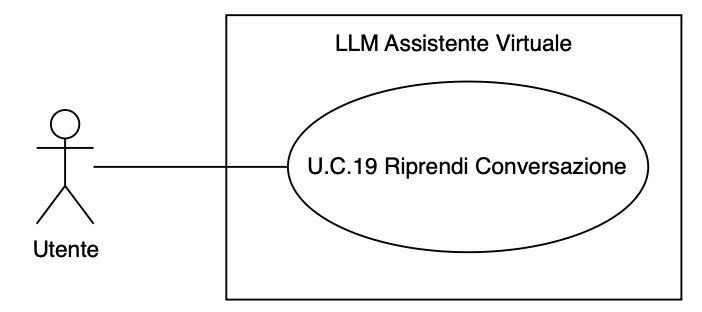
\includegraphics[width=0.7\textwidth]{img/UC19.png}
    \caption{U.C.19: Riprendi Conversazione}
\end{figure}
\newpage

\subsubsection{U.C.20: Risposta alla Richiesta dall’Amministratore}
\begin{itemize}
    \item \textbf{Attore}: Admin
    \item \textbf{Precondizioni}: L’amministratore ha effettuato l’accesso al sistema e in seguito alla dashboard per la gestione delle richieste di contatto. È presente almeno una richiesta inviata da un utente.
    \item \textbf{Postcondizioni}: L’amministratore ha risposto alla richiesta tramite email.
    \item \textbf{Scenario principale}: L’amministratore accede alla dashboard, seleziona una richiesta da gestire e ne visualizza i dettagli. Compone una risposta e la invia tramite il sistema.
    \item \textbf{Generalizzazioni}: -
    \item \textbf{Estensioni}: -
    \item \textbf{Inclusione}: -
\end{itemize}
\begin{figure}[H]
    \centering
    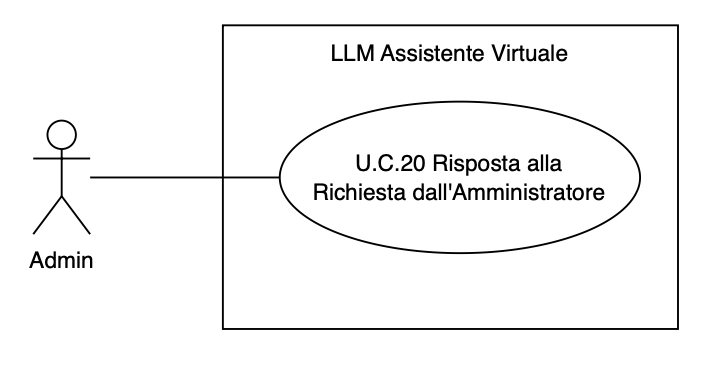
\includegraphics[width=0.7\textwidth]{img/UC20.png}
    \caption{U.C.20: Risposta alla Richiesta dall’Amministratore}
\end{figure}
\newpage

\subsubsection{U.C.21: Cambio stato Richiesta}
\begin{itemize}
    \item \textbf{Attore}: Admin
    \item \textbf{Precondizioni}: L’amministratore ha effettuato l’accesso al sistema e in seguito alla dashboard per la gestione delle richieste di contatto. È presente almeno una richiesta inviata da un utente.
    \item \textbf{Postcondizioni}: La richiesta è stata aggiornata come "gestita" dallo stato di “attesa”.
    \item \textbf{Scenario principale}: Dopo la risposta L’amministratore può decidere se lasciare la richiesta in stato di attesa o segnarla come “gestita”.
    \item \textbf{Generalizzazioni}: -
    \item \textbf{Estensioni}: -
    \item \textbf{Inclusione}: -
\end{itemize}
\begin{figure}[H]
    \centering
    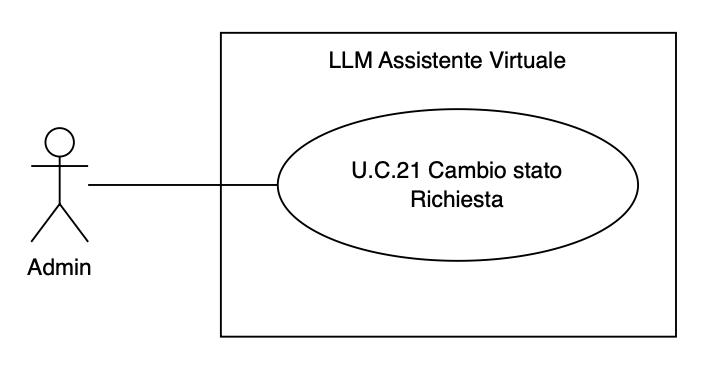
\includegraphics[width=0.7\textwidth]{img/UC21.png}
    \caption{U.C.21: Cambio stato Richiesta}
\end{figure}
\newpage

%% caso 21
\subsubsection{U.C.22 Invio Richiesta a un Operatore Umano}
\begin{itemize}
    \item \textbf{Attore}: Utente
    \item \textbf{Precondizioni}: L’utente ha ricevuto una risposta non soddisfacente dal sistema basato su \href{https://code7crusaders.github.io/docs/RTB/documentazione_interna/glossario.html#llm-large-language-model}{\textit{LLM}\textsuperscript{G}}.
    \item \textbf{Postcondizioni}: La richiesta dell’utente è stata inviata agli amministratori ed è visibile nella dashboard.    .
    \item \textbf{Scenario principale}: L’utente seleziona l’opzione per richiedere assistenza a un operatore umano, compila un modulo opzionale con eventuali dettagli e invia la richiesta. Il sistema registra la richiesta e la rende disponibile nella dashboard degli amministratori.
    \item \textbf{Generalizzazioni}: -
    \item \textbf{Estensioni}: -
    \item \textbf{Inclusione}: -
\end{itemize}
\begin{figure}[H]
    \centering
    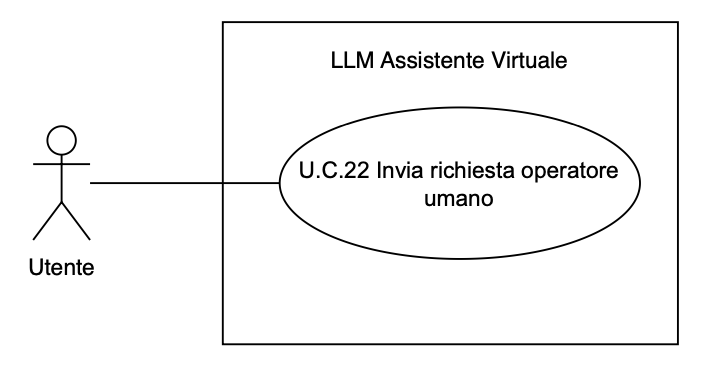
\includegraphics[width=0.7\textwidth]{img/UC22.png}
    \caption{U.C.22 Invio Richiesta a un Operatore Umano}
\end{figure}
\newpage

\newpage

\section{Requisiti}
In questa sezione vengono presentati i requisiti emersi durante l'attività di analisi, 
condotta a partire dai casi d'uso, dall'esame del capitolato d'appalto e dagli incontri, 
sia interni che con il proponente. 

\subsection{Classificazione dei requisiti}
I requisiti sono classificati in tre categorie principali:  
\begin{itemize}
    \item \textbf{Funzionali}: riguardano l'usabilità del prodotto finale;  
    \item \textbf{Di qualità}: includono gli strumenti e la documentazione da fornire;  
    \item \textbf{Di vincolo}: fanno riferimento alle tecnologie da utilizzare.
\end{itemize}
Per ciascun requisito è indicato:
\begin{itemize}
    \item \textbf{Codice Identificativo}: codice univoco che identifica il requisito;
    \item \textbf{Descrizione}: breve spiegazione del requisito;
    \item \textbf{Fonte}: origine del requisito (es. capitolato, interno, ecc..);
    \item \textbf{Priorità}: importanza del requisito rispetto agli altri;
\end{itemize} 

\subsection{Fonti dei requisiti}
I requisiti sono stati identificati a partire dalle seguenti fonti:
\begin{itemize}
    \item \textbf{Capitolato}: Requisiti individuati tramite analisi del capitolato;
    \item \textbf{interno}: requisiti individuati durante riunioni interne al gruppo di lavoro;
    \item \textbf{Esterno}: requisiti individuati durante incontri con il proponente;
    \item \textbf{Piano di Qualifica}: Requisiti necessari per rispettare standard di qualità definiti nel documento Piano di Qualifica;
    \item \textbf{Norme di Progetto}: Requisiti necessari per rispettare le norme di progetto definite nel documento Norme di Progetto;
\end{itemize}

\subsection{Codifica dei requisiti}
I requisiti sono codificati come segue: \textbf{R[Tipo][Importanza][Numero]}
\newline
Dove \textbf{Tipo} può essere:
\begin{itemize}
    \item \textbf{F (funzionale)}
    \item \textbf{Q (di qualità)}
    \item \textbf{V (di vincolo)}
\end{itemize}
\textbf{Importanza} può essere:
\begin{itemize}
    \item \textbf{O (obbligatorio)}
    \item \textbf{D (desiderabile)}
    \item \textbf{F (facoltativo )}
\end{itemize}
\textbf{Numero} è un numero identificativo univoco del requisito.

\textbf{Esempio}:
\begin{itemize}
    \item RFO1: Requisito funzionale obbligatorio numero 1
    \item RQD2: Requisito di qualità desiderabile numero 2
    \item RVF3: Requisito di vincolo facoltativo numero 3
\end{itemize}

\pagebreak
\subsection{Requisiti funzionali}
\begin{longtable}{|>{\centering\arraybackslash}m{0.10\textwidth}|>{\centering\arraybackslash}m{0.20\textwidth}|>{\centering\arraybackslash}m{0.6\textwidth}|}
	\hline
	\textbf{Codice} & \textbf{Fonte} & \textbf{Descrizione}\\\hline
	\endfirsthead
	\hline
	\textbf{Codice} & \textbf{Fonte} & \textbf{Descrizione}\\\hline
	\endhead
	\hline
	RFO1            & Capitolato    & Requisito funzionale obbligatorio numero 1
	\\\hline
	\caption{Requisiti funzionali}
\end{longtable}

\pagebreak
\subsubsection{Requisiti Qualitativi}
\begin{longtable}{|>{\centering\arraybackslash}m{0.10\textwidth}|>{\centering\arraybackslash}m{0.20\textwidth}|>{\centering\arraybackslash}m{0.6\textwidth}|}
	\hline
	\textbf{Codice} & \textbf{Fonte} & \textbf{Descrizione}\\\hline
	\endfirsthead
	\hline
	\textbf{Codice} & \textbf{Fonte} & \textbf{Descrizione}\\\hline
	\endhead
	\hline
	RQD2            & Interno    & Requisito di qualità desiderabile numero 2
	\\\hline
	\caption{Requisiti Qualitativi}
\end{longtable}

\pagebreak
\subsubsection{Requisiti di vincolo}
\begin{longtable}{|>{\centering\arraybackslash}m{0.10\textwidth}|>{\centering\arraybackslash}m{0.20\textwidth}|>{\centering\arraybackslash}m{0.6\textwidth}|}
	\hline
	\textbf{Codice} & \textbf{Fonte} & \textbf{Descrizione}\\\hline
	\endfirsthead
	\hline
	\textbf{Codice} & \textbf{Fonte} & \textbf{Descrizione}\\\hline
	\endhead
	\hline
	RVF3            & Esterno    & Requisito di vincolo facoltativo numero 3
	\\\hline
	\caption{Requisiti di vincolo}
\end{longtable}

\subsubsection{Requisiti sistema operativo}

\subsubsection{Requisiti di prestazione}

\subsubsection{Requisiti di sicurezza}

\pagebreak
\subsection{Tracciamento}
\subsubsection{Requisito - Fonte}
\begin{longtable}{|>{\centering\arraybackslash}m{0.40\textwidth}|>{\centering\arraybackslash}m{0.4\textwidth}|}
	\hline
	\textbf{Requisito} & \textbf{Fonte} 
	\endfirsthead
	\hline
	\textbf{Requisito} & \textbf{Fonte} 
	\endhead
	\hline
	RFO1            & Capitolato    
	\\\hline
    RQD2            & Interno
    \\\hline
    RVF3            & Esterno
    \\\hline
	\caption{Requisito - Fonte}
\end{longtable}




\end{document}
